\section{Security games of DSE schemes} \label{append:secGames}
Figure~\ref{fig:games} shows the $\Real^{\textsf{DSE}}$ and $\Ideal^{\textsf{DSE}}$ games for the DSE security definition~\ref{def:adpSec}.

\begin{figure}[!h]
	%\begin{tabular}[ll]
	%\centering
% 	\begin{figure}%[b]{0.5\textwidth}
	%\centering
	\begin{mdframed}
 %\begin{multicols}{1}
		\underline{$b\leftarrow \Real^{\textsf{DSE}}_{\text{Adv}}(\lambda, q)$:} 
		\begin{algorithmic}[1]
		    
			\State $N\leftarrow\A(1^\lambda)$ 
			\State $(K,\sigma_0, EDB_0) \leftarrow $\Setup$(1^\lambda, N)$
			%\algrenewcommand\algorithmicindent{0.5em}%
			\For{$k=1$ to $q$}
			%\algrenewcommand\algorithmicindent{-0.3em}%
			\State \hspace{-3pt}$(type_k,id_k,w_k)\leftarrow\A(1^\lambda,EDB_0,t_1,\ldots,t_{k-1})$
			\If{$type_k=search$}
			\State $(\sigma_k,DB(w_k);EDB_k) \leftarrow $\Search$(K,w_k,$
			\Statex \hspace{+5.3cm}$\sigma_{k-1};EDB_{k-1})$
			\ElsIf{$type_k=update$}
			%\algrenewcommand\algorithmicindent{18.0em}%
			\State \begin{varwidth}[t]{\linewidth}
				{$(\sigma_k;EDB_k) \leftarrow $\Update$(K,add/del,(id_k,w_k),$
				\Statex \hspace{+4.1cm} $\sigma_{k-1};$}
				%\par
				%\hskip\algorithmicindent 
				{$EDB_{k-1})$}
			\end{varwidth}			
			\EndIf
			\State Let $t_k$ be the messages from client to server in 
			\Statex \hspace{0.565cm}the $Search/Update$ protocols above
			%$Access$ protocol above
			\EndFor
			\State $b\leftarrow \A(1^\lambda,EDB_0,t_1,t_2,\ldots,t_q)$;
			\State \textbf{return} $b$;\newline
		\end{algorithmic}
		\underline{$b\leftarrow \Ideal^{\textsf{DSE}}_{\text{Adv}, Sim, \mathcal{L}}(\lambda, q)$:} 
		\begin{algorithmic}[1]
			\State $N\leftarrow\A(1^\lambda)$ 
			\State $(st_\mathcal{S},EDB_0)\leftarrow $SimSetup$(1^\lambda, N)$
			%\algrenewcommand\algorithmicindent{0.5em}%
			\For{$k=1$ to $q$}
			%\algrenewcommand\algorithmicindent{-0.3em}%
			\State  \hspace{-3pt}$(type_k,id_k,w_k)\leftarrow\A(1^\lambda,EDB_0,t_1,\ldots,t_{k-1})$
			\If{$type_k=search$}
			\State $(st_\mathcal{S};t_k,EDB_k) \leftarrow $SimSearch$(st_\mathcal{S},$
			\Statex \hspace{+4.4cm}$\mathcal{L}^{Srch}(w_k);EDB_{k-1})$
			\ElsIf{$type_k=update$}
			\State $(st_\mathcal{S};t_k,EDB_k)\leftarrow $SimUpdate$(st_\mathcal{S},$
			\Statex \hspace{+4.4cm}$\mathcal{L}^{Updt}(w_k);EDB_{k-1})$
			\EndIf
			\EndFor
			\State $b\leftarrow \A(1^\lambda,EDB_0,t_1,t_2,\ldots,t_q)$;
			\State \textbf{return} $b$
   %\Statex
		\end{algorithmic}
 % \end{multicols}
	\end{mdframed}
	%\vspace{-.5cm}
	\caption{Real and ideal experiments for the DSE scheme.}\label{fig:games}
	%\vspace{-.3cm}
\end{figure}


\section{Leakage Functions and Backward Privacy} \label{append:BP}
We need to describe some additional leakage functions to describe backward privacy. Let, list $Q$ has one entry for each query executed by the client. The entry for a search is of the form $(u,w)$ where $u$ is the query timestamp and $w$ is the searched keyword. The entry for an update is $(u, op, id)$ where $op = add/delete$ and $id$ is the modified file identifier. For a keyword $w$, let $TimeDB(w)$ be a function that returns the list of all (timestamp, file-identifier) pairs of keyword $w$ that have been added to $DB$ and have not been subsequently deleted, i.e. \newline
%\begin{align*}
    $TimeDB(w) =   \{(u, id)  | (u, add,,(w, id)) \in Q \wedge  \\
    ~~~~~~~~~~~~~~~~~~~~~~~~\forall u',(u', del, (w,id)) \notin Q \}$
%\end{align*}
\newline
$Updates(w)$ is a function that returns the timestamp of all insertion and deletion operations for $w$ in $Q$, i.e. \newline
$   Updates(w) =  \{u|(u, add, (w,id)) \in Q ~or~  
   (u, del, (w,id)) \\  ~~~~~~~~~~~~~~~~~~~~~~~~~~~~~~~~~~~~~~~~~~~~~~~~~~~~~~~~~~~~~~~~~~~~~~~~\in Q \}$
\newline
$DelHist(w)$ is a function that returns the history of deleted entries by revealing the insertion timestamp - deletion timestamp pairs (i.e. which deletion corresponds to which addition).
\newline
%\begin{align*}
    $DelHist(w) = \{(u^{add},u^{del} ) | \exists id : (u^{add}, add, (w,id)) \in Q \\ 
    ~~~~~~~~~~~~~~~~~~~~~~~~~~~~~~~~~~~~~~~~~~~~~~  ~ and ~ (u^{del} , del, (w,id)) \in Q \}$
%\end{align*}
\newline
Using the above functions, the three types of backward privacy is defined \cite{bost2017forward} as follows: \newline
%\begin{description}
\textbf{BP-I (BP with insertion pattern):}
    iff  $\mathcal{L}^{Updt}(op, w, id) = \mathcal{L}'(op)$ and 
    $\mathcal{L}^{Srch}(w) = \mathcal{L}''(TimeDB(w), n_w)$, \newline 
\textbf{BP-II (BP with update pattern):} 
    iff $\mathcal{L}^{Updt}(op, w, id) = \mathcal{L}'(op, w)$
    and     $\mathcal{L}^{Srch}(w) = \mathcal{L}''(TimeDB(w), Updates(w))$,\newline
\textbf{BP-III (weak BP):}  
iff $\mathcal{L}^{Updt}(op, w, id) = \mathcal{L}'(op, w)$ and 
$\mathcal{L}^{Srch}(w) = \mathcal{L}''(TimeDB(w), DelHist(w))$\newline
%\end{description}
Here $\mathcal{L}'$ and $\mathcal{L}''$ are two stateless functions and $n_w$ is 
total number of updates on $w$. 

\section{Oblivious Maps ($\textsc{OMAP}$).}\label{append:omap}
An oblivious map is a data structure that supports oblivious read/get and write/put functionality for encrypted $(key,value)$ pairs (i.e., oblivious hash map). That is, all same-length operation sequences appear indistinguishable. $\textsc{OMAP}$ has the following algorithms/protocols: (i) $\textsc{OMAP}$.$\texttt{Setup}$ initializes an empty data structure with maximum capacity $N$ blocks, (ii) $\textsc{OMAP}$.$\texttt{put}$ adds/overwrites a $(key,value)$ pair, and (iii) $\textsc{OMAP}$.$\texttt{get}$ returns the $value$ of a given $key$. We have used the AVL tree based implementation by Wang et al.~\cite{wang2014oblivious} on top of PathORAM~\cite{stefanov2013path}. For a map with capacity $N$, each oblivious access requires $\bO(\log^2 N)$ operations/accessed-blocks, $\bO(\log N)$ roundtrips, and $\bO(\log^2 N)$ locality---see~\cite{wang2014oblivious} for more details. 


\if 0
\paragraph{\textbf{Tethys}.}
Bossuat et al. \cite{BFF21} presented the first Page Efficient Searchable Encryption scheme (PE-SE) called \textsf{Tethys}.  This scheme offers $\bO(1)$ \emph{page efficiency} and $\bO(1)$ \emph{space overhead}.
For $N$ input items, this scheme allocates $m={(2+\epsilon){\cdot}N/p}$ pages, where $p$ is the memory page size and $\epsilon(>0)$ is a small arbitrary constant. For each keyword two pages are chosen using two hash functions $H_1$ and $H_2$. The set of pages returned by $H_1$ and $H_2$ are mutually exclusive. The entries are stored in the pages returned by $H_1$ and $H_2$, or in a stash at the client when page overflow occurs. An algorithm called data independent packing (DIP) is used to decide where the elements for a particular keyword are stored. The DIP algorithm makes sure that the load of each page is at most $p$, and at the same time it minimizes the size of the client stash. The authors proved that the size of the stash, i.e. the client storage is $\bO(p{\cdot}\omega(\log \lambda)/\log m)$. During search the two pages returned by $H_1$ and $H_2$ are fetched from the server and the stash is also searched. The keyword-lists that are larger than $p$ are divided into lists of size $p$, and they are stored and searched as independent lists. 
\fi


\begin{figure}[!h]
\centering
\scalebox{0.5}{
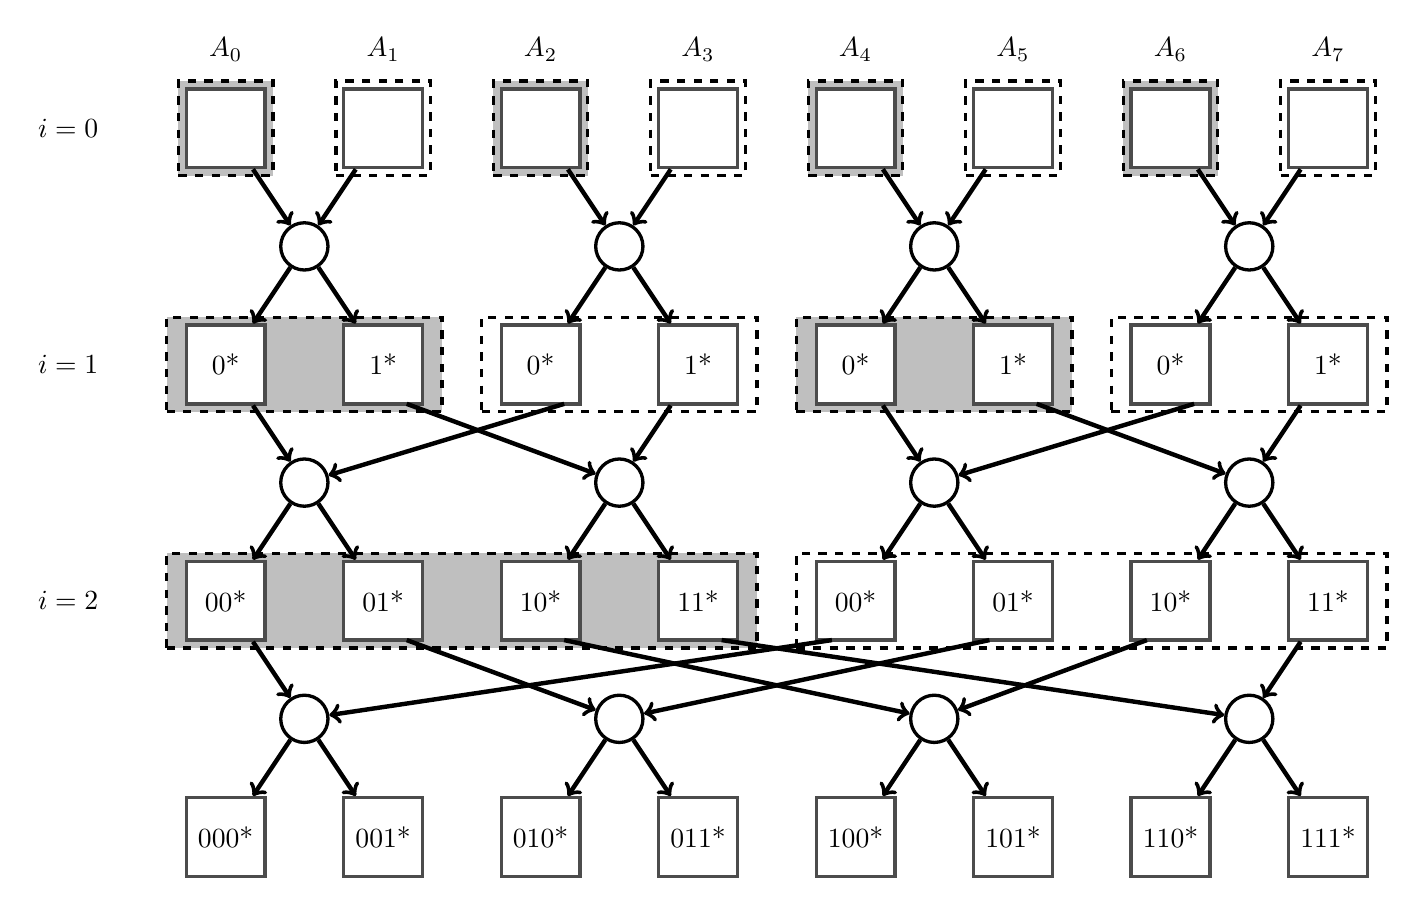
\begin{tikzpicture}
[
sq/.style={rectangle, draw=black!70, fill=white, very thick, minimum height=1cm, minimum width = 1cm},
textbox/.style={rectangle, draw=white, fill=white, very thick, minimum height=2.5cm},
box1/.style={rectangle, draw=black,dashed, fill=white, very thick, minimum height=1.2cm, minimum width=1.2cm},
box4/.style={rectangle, draw=black,dashed, fill=gray!50, very thick, minimum height=1.2cm, minimum width=1.2cm},
box2/.style={rectangle, draw=black,dashed, fill=white, very thick, minimum height=1.2cm, minimum width=3.5cm},
box5/.style={rectangle, draw=black,dashed, fill=gray!50, very thick, minimum height=1.2cm, minimum width=3.5cm},
box3/.style={rectangle, draw=black,dashed, fill=white, very thick, minimum height=1.2cm, minimum width=7.5cm},
box6/.style={rectangle, draw=black,dashed, fill=gray!50, very thick, minimum height=1.2cm, minimum width=7.5cm},
merge/.style={circle, draw=black, fill=white, very thick, minimum size=6mm},
myarrow1/.style={single arrow, draw=black, fill=black, 
      minimum width = 1mm, single arrow head extend=1mm,
      minimum height=1cm},
myarrow2/.style={single arrow, draw=red, fill=red, 
      minimum width = 1mm, single arrow head extend=1mm,
      minimum height=1.3cm},
myarrow3/.style={single arrow, draw=blue, fill=blue, 
minimum width = 0.09cm, single arrow head extend=0.05cm,
minimum height=0.7cm},
textbox/.style={rectangle, draw=white, fill=white, thick, minimum height=0.2cm},
]

\node at (0,6) [textbox] (t0) {$A_0$};
\node at (2,6) [textbox] (t0) {$A_1$};
\node at (4,6) [textbox] (t0) {$A_2$};
\node at (6,6) [textbox] (t0) {$A_3$};
\node at (8,6) [textbox] (t0) {$A_4$};
\node at (10,6) [textbox] (t0) {$A_5$};
\node at (12,6) [textbox] (t0) {$A_6$};
\node at (14,6) [textbox] (t0) {$A_7$};
\node at (-2,5) [textbox] (t0) {$i=0$};
\node at (-2,2) [textbox] (t0) {$i=1$};
\node at (-2,-1) [textbox] (t0) {$i=2$};

\node at (0,5) [box4] (b4) {} ;
\node at (0,5) [sq] (sq11) {};
\node at (2,5) [box1] (b4) {} ;
\node at (2,5) [sq] (sq12) {};
\node at (4,5) [box4] (b4) {} ;
\node at (4,5) [sq] (sq13) {};
\node at (6,5) [box1] (b4) {} ;
\node at (6,5) [sq] (sq14) {};
\node at (8,5) [box4] (b4) {} ;
\node at (8,5) [sq] (sq15) {};
\node at (10,5) [box1] (b4) {} ;
\node at (10,5) [sq] (sq16) {};
\node at (12,5) [box4] (b4) {} ;
\node at (12,5) [sq] (sq17) {};
\node at (14,5) [box1] (b4) {} ;
\node at (14,5) [sq] (sq18) {};

\node at (1,2) [box5] (b4) {} ;
\node at (0,2) [sq] (sq21) {0*};
\node at (2,2) [sq] (sq22) {1*};
\node at (1,3.5) [merge] (c11) {};
\draw[->,black, ultra thick]  (c11) -- (sq21);%(0.5,6.7) -- (1,6);
\draw[->,black, ultra thick]  (c11) -- (sq22);

\node at (5,2) [box2] (b4) {} ;
\node at (4,2) [sq] (sq23) {0*};
\node at (6,2) [sq] (sq24) {1*};
\node at (5,3.5) [merge] (c12) {};
\draw[->,black, ultra thick]  (c12) -- (sq23);
\draw[->,black, ultra thick]  (c12) -- (sq24);


\node at (9,2) [box5] (b4) {} ;
\node at (8,2) [sq] (sq25) {0*};
\node at (10,2) [sq] (sq26) {1*};
\node at (9,3.5) [merge] (c13) {};
\draw[->,black, ultra thick]  (c13) -- (sq25);
\draw[->,black, ultra thick]  (c13) -- (sq26);

\node at (13,2) [box2] (b4) {} ;
\node at (12,2) [sq] (sq27) {0*};
\node at (14,2) [sq] (sq28) {1*};
\node at (13,3.5) [merge] (c14) {};

\draw[->,black, ultra thick]  (c14) -- (sq27);
\draw[->,black, ultra thick]  (c14) -- (sq28);
\draw[->,black, ultra thick]  (sq11) -- (c11);
\draw[->,black, ultra thick]  (sq12) -- (c11);
\draw[->,black, ultra thick]  (sq13) -- (c12);
\draw[->,black, ultra thick]  (sq14) -- (c12);
\draw[->,black, ultra thick]  (sq15) -- (c13);
\draw[->,black, ultra thick]  (sq16) -- (c13);
\draw[->,black, ultra thick]  (sq17) -- (c14);
\draw[->,black, ultra thick]  (sq18) -- (c14);

\node at (3,-1) [box6] (b4) {} ;
\node at (0,-1) [sq] (sq31) {00*};
\node at (2,-1) [sq] (sq32) {01*};
\node at (1,0.5) [merge] (c21) {};
\draw[->,black, ultra thick]  (c21) -- (sq31);
\draw[->,black, ultra thick]  (c21) -- (sq32);
\node at (4,-1) [sq] (sq33) {10*};
\node at (6,-1) [sq] (sq34) {11*};
\node at (5,0.5) [merge] (c22) {};
\draw[->,black, ultra thick]  (c22) -- (sq33);
\draw[->,black, ultra thick]  (c22) -- (sq34);
\node at (11,-1) [box3] (b4) {} ;
\node at (8,-1) [sq] (sq35) {00*};
\node at (10,-1) [sq] (sq36) {01*};
\node at (9,0.5) [merge] (c23) {};
\draw[->,black, ultra thick]  (c23) -- (sq35);
\draw[->,black, ultra thick]  (c23) -- (sq36);
\node at (12,-1) [sq] (sq37) {10*};
\node at (14,-1) [sq] (sq38) {11*};
\node at (13,0.5) [merge] (c24) {};
\draw[->,black, ultra thick]  (c24) -- (sq37);
\draw[->,black, ultra thick]  (c24) -- (sq38);
\draw[->,black, ultra thick]  (sq21) -- (c21);
%\draw[->,black, ultra thick]  (5.4,2) -- (c21);
%\draw[->,black, ultra thick]  (2.6,2) -- (c22);
\draw[->,black, ultra thick]  (sq24) -- (c22);
\draw[->,black, ultra thick]  (sq25) -- (c23);
%\draw[->,black, ultra thick]  (17.8,2) -- (c23);
%\draw[->,black, ultra thick]  (15.6,2) -- (c24); 
\draw[->,black, ultra thick]  (sq28) -- (c24);

\draw[->,black, ultra thick]  (2.3,1.5) -- (c22);%%
\draw[->,black, ultra thick]  (4.3,1.5) -- (c21);%%
\draw[->,black, ultra thick]  (10.3,1.5) -- (c24);%%
\draw[->,black, ultra thick]  (12.3,1.5) -- (c23);%%

\node at (0,-4) [sq] (sq41) {000*};
\node at (2,-4) [sq] (sq42) {001*};
\node at (1,-2.5) [merge] (c31) {};
\draw[->,black, ultra thick]  (c31) -- (sq41);
\draw[->,black, ultra thick]  (c31) -- (sq42);
\node at (4,-4) [sq] (sq43) {010*};
\node at (6,-4) [sq] (sq44) {011*};
\node at (5,-2.5) [merge] (c32) {};
\draw[->,black, ultra thick]  (c32) -- (sq43);
\draw[->,black, ultra thick]  (c32) -- (sq44);
\node at (8,-4) [sq] (sq45) {100*};
\node at (10,-4) [sq] (sq46) {101*};
\node at (9,-2.5) [merge] (c33) {};
\draw[->,black, ultra thick]  (c33) -- (sq45);
\draw[->,black, ultra thick]  (c33) -- (sq46);
\node at (12,-4) [sq] (sq47) {110*};
\node at (14,-4) [sq] (sq48) {111*};
\node at (13,-2.5) [merge] (c34) {};
\draw[->,black, ultra thick]  (c34) -- (sq47);
\draw[->,black, ultra thick]  (c34) -- (sq48);
\draw[->,black, ultra thick]  (sq31) -- (c31);%

\draw[->,black, ultra thick]  (7.7,-1.5) -- (c31);
\draw[->,black, ultra thick]  (2.3,-1.5) -- (c32);
\draw[->,black, ultra thick]  (9.7,-1.5) -- (c32);
\draw[->,black, ultra thick]  (4.3,-1.5) -- (c33);
\draw[->,black, ultra thick]  (11.7,-1.5) -- (c33);
\draw[->,black, ultra thick]  (6.3,-1.5) -- (c34);

\draw[->,black, ultra thick]  (sq38) -- (c34); %
\end{tikzpicture}
}
\captionsetup{font=small}
\caption{Oblivious random bin assignment with 8 buckets: The circles \textbf{\textbigcircle}\ denote 
the \textsf{MergeSplit} units and the squares \textbf{\large{$\square$}}\ denote buckets. 
The \mergeSplit\ function takes two buckets at level $i$ 
and put them into two consecutive buckets at level $i+1$, based on 
the $(i+1)th$ most significant bit of the random keys assigned to each element of the buckets. 
This figure is replicated from Figure 1 of [5].}
\label{fig:bucketSort}
\end{figure}

\begin{figure}[!h]
\centering
\scalebox{0.5}{
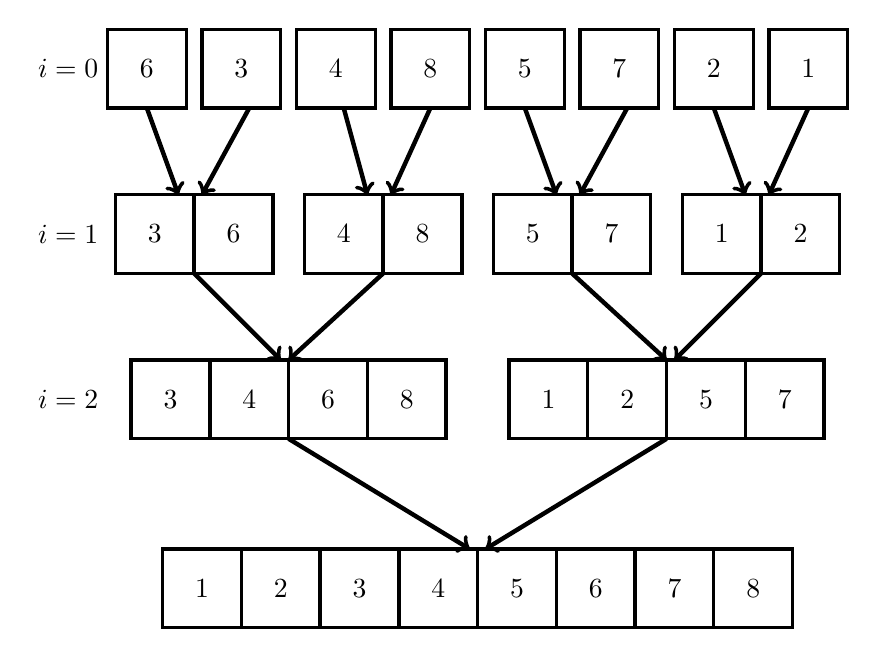
\begin{tikzpicture}
[
sq/.style={rectangle, draw=black!70, fill=white, very thick, minimum height=2cm, minimum width = 2cm},
textbox/.style={rectangle, draw=white, fill=white, very thick, minimum height=2.5cm},
box1/.style={rectangle, draw=black, fill=white, very thick, minimum height=1cm, minimum width=1cm},
merge/.style={circle, draw=black, fill=white, very thick, minimum size=8mm},
myarrow1/.style={single arrow, draw=black, fill=black, 
      minimum width = 1mm, single arrow head extend=1mm,
      minimum height=1cm},
textbox/.style={rectangle, draw=white, fill=white, thick, minimum height=0.2cm},
]

\node at (-1,0) [textbox] (t1) {$i=0$};
\node at (-1,-2.1) [textbox] (t2) {$i=1$};
\node at (-1,-4.2) [textbox] (t3) {$i=2$};

\node at (0,0) [box1] {6};
\node at (1.2,0) [box1] {3};
\node at (2.4,0) [box1] {4};
\node at (3.6,0) [box1] {8};
\node at (4.8,0) [box1] {5};
\node at (6,0) [box1] {7};
\node at (7.2,0) [box1] {2};
\node at (8.4,0) [box1] {1};

\node at (0.1,-2.1) [box1] {3};
\node at (1.1,-2.1) [box1] {6};
\node at (2.5,-2.1) [box1] {4};
\node at (3.5,-2.1) [box1] {8};
\node at (4.9,-2.1) [box1] {5};
\node at (5.9,-2.1) [box1] {7};
\node at (7.3,-2.1) [box1] {1};
\node at (8.3,-2.1) [box1] {2};

\node at (0.3,-4.2) [box1] {3};
\node at (1.3,-4.2) [box1] {4};
\node at (2.3,-4.2) [box1] {6};
\node at (3.3,-4.2) [box1] {8};
\node at (5.1,-4.2) [box1] {1};
\node at (6.1,-4.2) [box1] {2};
\node at (7.1,-4.2) [box1] {5};
\node at (8.1,-4.2) [box1] {7};

\node at (0.7,-6.6) [box1] {1};
\node at (1.7,-6.6) [box1] {2};
\node at (2.7,-6.6) [box1] {3};
\node at (3.7,-6.6) [box1] {4};
\node at (4.7,-6.6) [box1] {5};
\node at (5.7,-6.6) [box1] {6};
\node at (6.7,-6.6) [box1] {7};
\node at (7.7,-6.6) [box1] {8};

\draw[->,black, ultra thick]  (0,-0.5) -- (0.4,-1.6);
\draw[->,black, ultra thick]  (1.3,-0.5) -- (0.7,-1.6);

\draw[->,black, ultra thick]  (2.5,-0.5) -- (2.8,-1.6);
\draw[->,black, ultra thick]  (3.6,-0.5) -- (3.1,-1.6);

\draw[->,black, ultra thick]  (4.8,-0.5) -- (5.2,-1.6);
\draw[->,black, ultra thick]  (6.1,-0.5) -- (5.5,-1.6);

\draw[->,black, ultra thick]  (7.2,-0.5) -- (7.6,-1.6);
\draw[->,black, ultra thick]  (8.4,-0.5) -- (7.9,-1.6);


\draw[->,black, ultra thick]  (0.6,-2.6) -- (1.7,-3.7);
\draw[->,black, ultra thick]  (3,-2.6) -- (1.8,-3.7);
\draw[->,black, ultra thick]  (5.4,-2.6) -- (6.6,-3.7);
\draw[->,black, ultra thick]  (7.8,-2.6) -- (6.7,-3.7);

\draw[->,black, ultra thick]  (1.8,-4.7) -- (4.1,-6.1);
\draw[->,black, ultra thick]  (6.6,-4.7) -- (4.3,-6.1);

\end{tikzpicture}
}
%\captionsetup{font=small}
\caption{Merge sort: always two consecutive chunks of $2^i$ elements from 
level $i$ are merged 
and written to $2^{i+1}$ consecutive memory locations at level $i+1$. 
%This causes 2 random disk-head movements for a single merge.
}
\label{fig:mergeSort}
\end{figure}

\section{De-amortizing bucket oblivious sort.} \label{append:bucketSort} \label{append:bucketLoc}
 An oblivious sorting algorithm sorts an array of elements without leaking information about the relative ordering of the input elements. 
 Recently, Asharov et al.~\cite{bucketSort} presented an oblivious bucket
 sort algorithm that obliviously sorts the input elements in three steps: First, it performs an \emph{Oblivious Random Bin Assignment} (ORBA). ORBA obliviously and uniformly randomly distribute the $N$ input elements and $N$ extra dummy elements into a set of buckets. Each element is assigned to an independent random bucket, and elements are then routed into the buckets obliviously. %Fetching one bucket from disk requires always $\bO(1)$ locality, since the elements of a bucket are always stored in contiguous memory locations. 
 Second, after performing the ORBA, it computes an \emph{Oblivious Random Permutation (ORP)}  which is achieved by scanning the output of ORBA, deleting dummy elements from each bin and then obliviously permuting each bin (either locally or using bitonic sort). Finally, it  sorts the ORP output using any \emph{non-oblivious} comparison-based sort.
 % We can de-amortize bucket sort into $N \log N/\gamma$ rounds of $\bO(\gamma)$ work per round (e.g., for $\gamma = O(\log N)$ the oblivious bucket sort can be completed in $N$ rounds---see Appendix \ref{append:bucketSort} for more details. 
 We use merge sort as the \emph{non-oblivious} sort. Merge-sort is a stable sort (preserves relative ordering of elements). %One merge operation in merge sort has $\bO(1)$ locality. 
 This algorithm takes $\bO(N\log N)$ time (assuming the client can safely store a small number of elements, e.g., for $N=2^{30}$ the client needs to store $1024$ elements locally). 
 \newline
 \underline{\textbf{De-amortizing Oblivious Random Bin Assignment}}
There are a total of $B= \frac{2{\cdot}N}{Z}$ buckets, where $Z$ is the size of the
buckets. In the bucket sort algorithm a total of $\log B$ levels of \mergeSplit s
(see Figure \ref{fig:bucketSort}) take place. 
And in each of these levels $\frac{B}{2}$ \mergeSplit s happen.
That is, overall $\frac{B}{2} {\cdot} \log B$ \mergeSplit s takes place. 
In, other words, one can de-amortize the oblivious random bin assignment 
in $\frac{B/2 {\cdot} \log B}{\gamma}$ steps, doing $\gamma$ \mergeSplit s in each step.
\newline
\underline{\textbf{De-amortizing Oblivious Random Permutation (ORP)}}
For this step the client fetches one bucket, 
removes all the dummy elements (which comes at the end) and locally permute the
non-dummy elements. 
As there are $B$ buckets, this step can be de-amortized
into at most of $B$ steps. If we permute $\gamma$ buckets in a single step then
ORP can be performed in $\frac{B}{\gamma}$ steps. 
\newline
\underline{\textbf{De-amortizing Non Oblivious sort}} 
We have used iterative merge sort in this step,
which can be de-amortized. 
For an input array of $N$ items merge sort runs in $\log N$ levels, 
and does $N$ work (compares) per level (see Figure \ref{fig:mergeSort}). 
The $ith$ level sorts every chunk of 
$2^i$ elements. Or in other words, the $ith$ level merges two consecutive 
sorted chunk of $2^{i-1}$ elements. If we de-amortized merge sort doing 
$\gamma$ work (merges) per step, it will require $\frac{N \log N}{\gamma}$ 
steps to finish the merge sort. \newline
%If $\gamma = {\log N$, the merge sort takes $N$ rounds
%to sort $N$ items. 
\underline{\textbf{Locality of bucket oblivious sort.} }
\textbf{(i)} Fetching a bucket from the disk requires one I/O, 
since the elements of the bucket are stored in contiguous memory locations.
Fetching two buckets during a single \mergeSplit\ will cause two I/Os. 
The outputs are written to two consecutive buckets, causing only one I/O. 
Hence, we can say the one \mergeSplit\ of {oblivious random 
bin assignment} (ORBA) causes three I/Os, or has $\bO(1)$ locality. 
Overall, there are $\frac{B}{2}{\cdot} \log B$ \mergeSplit s, and hence
$\bO(B \log B) < \bO(N \log N)$ locality.
\textbf{(ii)} For the ORP, fetching one bucket causes one I/O. 
The permuted elements are written back 
to consecutive memory locations, which causes another I/O. 
There are $B$ buckets, hence the ORP causes $2{\cdot} B$ 
random disk-head movement in total. 
So, one step of ORP has $\bO(1)$ locality and overall ORP has $\bO(B)$ 
locality. \textbf{(iii)} During a particular merge in merge sort, 
two consecutive chunks of $2^i ~(0 \leq i \leq (\log N-1))$ elements are fetched, 
sorted and the merged output is written back to $2^{i+1}$ consecutive 
memory locations. In this way, one merge costs two I/Os. 
There are $\log N$ levels, where the level $i$ requires 
$2^{{\log N}}$ random I/Os; taking summation of all these we get merge sort's 
locality to be $\bO(N)$. This makes locality of bucket oblivious sort to be 
$\bO(N \log N)$.


\section{Definitions of I/O efficiency metrices.} \label{append:metrics}

\begin{definition}[Search locality]
\neww{The search locality (or locality) of an SE scheme (static or dynamic) that uses HDDs as the underlying storage medium is defined as the total number of non-contiguous memory regions read during a search operation.  } 
\end{definition}

\begin{definition}[Update locality]
\neww{The update locality of a DSE scheme that uses HDDs as the underlying storage medium is defined as the total number of non-contiguous memory regions accessed during an update operation.  } 
\end{definition}

\begin{definition}[Read efficiency]
\neww{The read efficiency of an SE scheme that uses HDDs as the underlying storage medium is defined as the ratio of total number of memory locations read over the number of memory locations read pertaining to the results during a search operation.}
\end{definition}

 %All of these three metrices are relevant for schemes that use HDDs as the storage medium.

\begin{definition}[Page efficiency]
The page efficiency of an SE scheme that uses SSDs as the underlying storage medium is defined as the ratio of the total number of memory pages read for encrypted result during a search over the number of memory pages that would have been read for the plaintext result.
\end{definition}

\begin{definition}[Update efficiency]
\neww{The page efficiency of a DSE scheme that uses SSDs as the underlying storage medium is defined as the number of memory pages accessed during an update operation.}
\end{definition}

\begin{definition}[Update asymptotic cost]
\neww{The update asymptotic cost of a DSE scheme that uses either HDDs or SSDs as the underlying storage medium is defined as the asymptotic cost of a single insert or a delete.}
\end{definition}

\begin{definition}[Space overhead]
\neww{The space overhead of an SE scheme that uses either HDDs or SSDs as the underlying storage medium is defined as the ratio of the total space used to store the encrypted database over the size of the plaintext database.}
\end{definition}

\neww{Search locality is commonly referred as just \emph{locality}. \emph{Read efficiency}, 
\emph{locality}, \emph{page efficiency} and \emph{space overhead} are applicable for both SSEs and DSEs, while \emph{update locality} and \emph{update asymptotic} cost are applicable only for DSEs.}


\begin{figure}[!h]
	\begin{mdframed}
		\setlength{\itemindent}{-.3 in}
		Let {\sf $\Gamma$ = (\Setup, \Search, \texttt{DecryptAll})} be a result-hiding, static searchable encryption scheme.
 %\begin{multicols}{2}
  \underline{$(K,\sigma , EDB) \leftarrow \Setup(\lambda,N)$}
		\begin{algorithmic}[1]
		\State Let $\ell \gets \lfloor \log N \rfloor$
		\FFor{$i=0\ldots \ell$} Set empty index $EDB_i$ of size $2^i$
			\State $EDB$  $\gets \{EDB_0, \ldots, EDB_\ell\}$
			\State Set $K,\sigma$ to be empty vectors
			\State \Return $EDB$ to Server and $(K,\sigma)$ to Client \newline
		\end{algorithmic}
		%\underline{$(st_{\sf C},\mathcal{I})\leftarrow${\sf Update}$(op,w,id,st_{\mathcal{C}})$}
		\underline {$(K, \sigma ; EDB) \leftrightarrow$ {\Update$(K,op,w,id,\sigma;EDB)$}}
		\begin{algorithmic}[1]
			\item[Server:]
			\State Find the minimum $j$ such that $EDB_j = \emptyset$
			\State Send to client $EDB_0,\dots,EDB_{j-1}$
			
			\item[Client:]
			\State Set $A \leftarrow \emptyset$
			\For{$i=0, \dots, j-1$}
			\State $A\leftarrow$ $A\; \cup$ {\sf $\Gamma$.\texttt{DecryptAll}}($K[i],\sigma[i],EDB_i$)
			\State $K[i] \leftarrow \bot$, $\sigma[i]\leftarrow \bot$
			\EndFor
			\State {\small $(K[j],\sigma[j],EDB_A) \leftarrow$} {\sf $\Gamma$.\Setup} {\small ($A \cup (w,id,op)$)}
				\State \Return $EDB_A$ to server
			\item[Server:]
			\State Set $EDB_j \leftarrow EDB_A$
			\For{$i=0, \dots, j-1$}
			\State Set $EDB_i \leftarrow \emptyset$
			\EndFor\newline
		\end{algorithmic}
		\underline{$DB(w) \leftrightarrow \textsf{\Search}(K,q,\sigma ; EDB)$}
		\begin{algorithmic}[1]
			\item[Client $\leftrightarrow$ Server:]
			\State $\mathcal{X}\leftarrow\emptyset$.
			\For{all $i$ such that $EDB_i\neq \emptyset$}
			\State Let $\mathcal{X}_i \leftrightarrow$ {\sf $\Gamma$.\Search}($K[i],q,\sigma[i]; EDB_i$)
			\State $\mathcal{X}\leftarrow \mathcal{X} \cup \mathcal{X}_i$
			\EndFor
			\State Send $\mathcal{X}$ to the Client
			\item[Client:]
			%\State Decrypt entries of $\mathcal{X}$ with $K$ and parse them as $(id,op)$
			\State $DB(w) \leftarrow \{id\; | \; (w,id,add)\in \mathcal{X} \land (w,id,del) \not\in \mathcal{X}\}$
			\State \Return $DB(w)$
			%\State \textbf{return} $(\mathcal{X},st_{\mathcal{C}}',\mathcal{I}')$.
		\end{algorithmic}
  %\end{multicols}
	\end{mdframed}
	%\vspace{-0.3cm}
	\caption{{\sf SD}$_a$: from static to dynamic (optimized version).\cite{SDa}}
	%\vspace{-.2cm}
	\label{fig:Scheme1}
\end{figure}

\section{\SDa[$\cdot$]: Details and efficiency proofs}\label{append:SDalocProofs}

The pseudocode of the optimized version of \SDa[$\cdot$] is presented in Figure \ref{fig:Scheme1}. Below we prove a theorem that says, when a \emph{locality-aware} 
static SE scheme $\Gamma$ instantiated with \SDa[$\cdot$] to produce a \emph{locality-aware} DSE scheme  \SDa[$\cdot$], it retains the original \emph{space-overhead} of $\Gamma$, but for \emph{read-efficiency} and \emph{locality} an additional factor of $\log N$ is introduced as each of $\log N$ indexes are queried separately.  

%\begin{restatable}{theorem}{SDaLoc}\label{thm:SDaLoc}
\begin{theorem}\label{thm:SDaLoc}
Assuming a database of size $N$, and a locality-aware static SE scheme $\Gamma$ 
with $\bO(S)$ space overhead, $\bO(R)$ {search} read-efficiency, 
and $\bO(L)$ {search} locality,
\SDa$[\Gamma]$ has $\bO(S)$ space overhead, $\bO(R+ \log N)$ 
{search} read-efficiency, $\bO(L+\log N)$ {search} locality.% ,  and $\bO(\log N)$ update locality. 
\end{theorem}
%\end{restatable}
%\vspace{-0.3cm}
%\noindent\textit{Proof.}
%\end{theorem}
\begin{proof}\label{thm:SDaLocProof}
 %See Appendix \ref{append:SDalocProofs}
%\SDaLoc* 
%\noindent\textit{Proof.}
\new{In \SDa[$\Gamma$], at most ${\log{N}}$ indices
are created for a database of size $N$. 
%Without loss of generality, 
%we will be using $\log{N}$ instead of $\ceil{\log{N}}$ in the rest of our proof.  
The $k$th index in \SDa[$\Gamma$] is an instance of the static 
SE scheme $\Gamma$ that stores $2^k$ elements. 
\newline 
%\newline
\noindent{\textbf{Space overhead.}} 
%Hence, each individual index in \SDa[$\Gamma$] 
Space overhead of $\Gamma$ is $\bO(S)$; i.e. 
the space complexity is $\bO(S \cdot N)$. %because $\Gamma$ has space overhead \bO(S)$. 
%if $\Gamma$ needs $\bO{(S{\cdot}N)}$ space, 
%then 
Hence, the total space required by \SDa[$\Gamma$] (for a positive constant $c$) is:  
%\begin{align*}
 $c \cdot (S{\cdot}2^0 + S{\cdot}2^1 + \ldots + S{\cdot}2^{\log N -1}) \leq  c{\cdot}S{\cdot}N =  \bO(S{\cdot}N)$

Which incurs $\bO(S)$ \emph{space overhead} for \SDa[$\Gamma$].
\newline%\newline
\noindent{\textbf{Search read efficiency.}} Let us assume keyword $w$ is 
associated to $n_w$ results. 
Because, $\Gamma$ has $\bO(R)$ \emph{search read efficiency}, 
during a search query of $w$, $\Gamma.\Search(K,w,\sigma;EDB)$ 
returns $\bO(R{\cdot}n_w)$ entries. 
%and $\bO(L)$ search locality respectively.
Now, in \SDa[$\Gamma$], those $n_w$ results can be distributed into $\log N$ indexes. 
%(during the updates and local merges). %for \SDa[$\Gamma$]. 
Let us assume that $EDB_k$ has $a_{w_k}$ entries, 
i.e. $0 \leq a_{w_k} \leq a_{w}~~\forall k \in \{0,\ldots,(\log N -1)\}$,
and $n_w = a_{w_0}+a_{w_1}+\ldots+a_{w_{(\log N-1)}}$. 
But, for every $k$th index $EDB_k$, 
the corresponding keyword dictionary (i.e. $EDB_k.\Dict$) 
is queried as well to get the keyword counter values for $w$. 
Hence, total amount of data read for is $EDB_k$ is $\bO(R{\cdot}a_{w_k} + 1)$,
 In \SDa[$\Gamma$], the search happens individually in every index by calling $\Gamma.\Search$.
% Hence the $k$th index returns $\bO(R{\cdot}{a_{w_k}}+1)$ entries. 
Taking the summation 
 of the total data read from all the indexes and dictionaries we get (for a constant $c$):
%\begin{align*}
 $c{\cdot}((R{\cdot}a_{w_0} +1 )+ (R{\cdot}a_{w_1}+1) + \ldots + (R{\cdot}a_{w_{\log N -1}}+1))
%\intertext{\hspace{3cm}$c$ being a constant}
%=& y{\cdot}R{\cdot}(a_{w_0} + a_{w_1} + \ldots +a_{w_{(\log N -1)}}) \\
=  c{\cdot}(R{\cdot}n_w +\log{N})  = \bO(R{\cdot}n_w + \log N)$
%\end{align*} 
which results into \emph{search read efficiency} to be
$\bO(R + \frac{\log N}{n_w})$  i.e.  $\bO(R+\log N)$
\newline %\newline
\noindent{\textbf{Search locality.}} A search query for keyword $w$ in $\Gamma$ causes $\bO(L)$ random 
disk head movements, as $\Gamma$ has $\bO(L)$ \emph{search locality}. 
Let us assume, for each $EDB_k$ in \SDa[$\Gamma$], the disk head moves $L_k$ times 
(which is at most $a_{w_k}$, if $\Gamma$ has worst case locality). So, disk head moves a total of 
$\Sigma_{0 \leq k \leq (\log N -1)} L_k = c{\cdot}L$ times (for some constant $c$). %which is at most $n_w$, if $\Gamma$ 
%has worst case locality.
%But $\Gamma$ has locality $\bO(L)$. 
Moreover, for each access to the dictionaries the disk head moves once, 
causing an extra $\log N$ random disk head movements. 
Hence, in total, \SDa[$\Gamma$] has $(c\cdot L + \log N )$  i.e. $\bO(L + \log N)$ locality.
}
\end{proof}

We have discussed about the potential static SE candidates in 
section \ref{sec:SDalocality}. Here, we will choose \SDa[\OneChoice] 
to explain the locality and read-efficiency as stated in the Theorem \ref{thm:SDaLoc} above.
 %,and on \SDa~with \Tethys, denoted \SDa[\Tethys].
The $i^{th}$ index of \SDa$[\OneChoice]$ stores the
real $2^i$ elements across $\ceil{{2^i}/{\log 2^i \log \log 2^i}}$ bins.
 During a search, each index is searched by calling 
\OneChoice.\Search, with locality $\bO(1)$, 
as \emph{locality} of \OneChoice\ is $\bO(1)$.
Since there are at most $\log N$ non-empty indexes: \new{$EDB_0.\Ind$, $EDB_1.\Ind$ \ldots $EDB_{\log N -1}.\Ind$, 
and the corresponding $\log N$ dictionaries: $EDB_0.\Dict$, $EDB_1.\Dict$ \ldots $EDB_{\log N-1}.\Dict$, the total number of required I/Os is $2\log N$, i.e.} search locality for \SDa$[\OneChoice]$ is $\bO(\log N)$. 
Read-efficiency for \SDa$[\OneChoice]$ is $\bO(\log N \log\log N + \log N)$; \new{the extra $\log N$ factor is added as $\log N$ keyword counter information is fetched from the $\log N$ dictionaries}. 
The transformation preserves the storage overhead of \OneChoice, which is optimal. %($\bO(N)$). 
Finally, regarding updates, the amortized update overhead is $\bO(\log N)$ as the setup time of \OneChoice~ is linear, and the update locality is $\bO(\log N)$ as at most $\log N$ indexes are fetched. Table~\ref{table:SDaLoc} provides different instantiations of the \SDa[$\cdot$] transformation with \emph{locality-aware} static SE schemes. We highlight that the amortized update overhead for \TwoChoice\ and \NlogN\ is $\bO(\log^2 N)$ since their setup time is $\bO(N \log N)$. 


Below we prove another theorem, for \emph{page-efficient} static SE schemes instantiated with \SDa[$\cdot$].

\begin{theorem}\label{thm:SDaPE}
Assuming a database of size $N$, and a page efficient static SE scheme $\Gamma$ 
with $\bO(P)$ page efficiency, and $\bO(S)$ space overhead,
\SDa$[\Gamma]$ has 
$\bO(S)$ space overhead, and $\bO(P + \log N)$ worst case search page efficiency. 
%\tblue{what about update efficiency?}.
\end{theorem}
%\end{theorem}
%\noindent\textit{Proof.} \tblue{See Appendix \ref{thm:SDaPEProof}}
%\vspace{-0.3cm}
\begin{proof}
\new{In \SDa[$\Gamma$], at most ${\log{N}}$ indices
are created for a database of size $N$. The $k$th index in \SDa[$\Gamma$] 
stores $2^k$ elements. 
\newline %\newline
\noindent{\textbf{Space overhead.}}
For a database with $N$ entries $\Gamma$ has $\bO(S)$ 
space overhead, i.e. it uses $\bO(\frac{S{\cdot}N}{p})$ pages,
where $p$ is the page size.
The total space required by \SDa[$\Gamma$] can be calculated in a similar fashion
to Theorem \ref{thm:SDaLoc}, i.e. 
%\begin{align*}
$c{\cdot}(\frac{S}{p}{\cdot}2^0 + \frac{S}{p}{\cdot}2^1 + \ldots \\
+ \frac{S}{p}{\cdot}2^{\log N -1}) \leq  c \cdot \frac{S}{p}{\cdot}N = \bO(S{\cdot}N)$
; which incurs $\bO(S)$ \emph{space overhead}.
\newline %\newline
\noindent{\textbf{Search page efficiency.}} 
$\Gamma$ has $\bO(P)$ \emph{search page efficiency}. Let us assume keyword $w$ has $n_w$ results. 
During a search query of $w$, $\Gamma.\Search(K,w,\sigma;EDB)$ returns $\bO(\frac{{P{\cdot}n_w}}{p})$ 
pages. % (for an integer constant $y$), 
%and it causes $z{\cdot}L$ random disk head movements, 
%and $\bO(L)$ search locality respectively.
The $n_w$ results can get distributed in $\log N$ indexes 
in \SDa[$\Gamma$]. Let us assume that $EDB_k$ has $a_{w_k}$ entries, 
for $0 \leq k \leq (\log N-1)$, i.e. $n_w$ = $a_{w_0}$$+a_{w_1}+$$\ldots+$$a_{w_{(\log N-1)}}$.
 In \SDa[$\Gamma$], the search happens individually in every index by calling $\Gamma.\Search$.
 Hence the $k$th index returns $\bO(\frac{P{\cdot}{a_{w_k}}}{p}+2)$ pages. 
 The extra 2 pages are returned 
 because in worst case the starting and ending point of the result list might not be page aligned. 
 Moreover, another page is fetched during querying the 
 keyword dictionary. Taking summation of all we get, (for some constant $c$):
%\begin{align*}
$ c{\cdot}(\frac{P{\cdot}a_{w_0}}{p} +3)+ (\frac{P{\cdot}a_{w_1}}{p} +3) + \ldots + (\frac{P{\cdot}a_{w_{\log N -1}}}{p} +3)\\
%=& \frac{P}{p}{\cdot}(r_0 + r_1 + \ldots +r_{(\log N -1)}) + 3{\cdot}\log N \\
=  \frac{c \cdot P}{p}{\cdot}n_w + 3 {\cdot} \log N $
%\end{align*} 
%The $\log N$ dictionaries are queried to get the keyword counters, that results 
%into fetching additional $\log N$ pages. Hence the total number of pages fetched are
%$\frac{y{\cdot}P}{p}{\cdot}r + 2 {\cdot} \log N$ + $\log N$, 
which makes the 
\emph{search page efficiency} to be $c\cdot (P + \frac{3{\cdot}\log N}{n_w/p})$ i.e. $\bO(P + \log N)$.}
\end{proof}

Static \emph{page-efficient} schemes, e.g., \Tethys\ \cite{BFF21} and \NlogN\ \cite{onechoice} can be instantiated with \SDa\. \Tethys\ fetches two pages from the server during search, hence it offers $\bO(1)$ \emph{search page efficiency}. The page efficiency of \SDa[\Tethys] will be $\bO(\log N)$ since it will require two page accesses per index.   
The amortized update overhead of \SDa[\Tethys] is $\bO(N \log N)$ 
since its setup time is $\bO(N^2)$. 
Similarly, the page efficiency of \SDa[\NlogN] is $\bO(\log N)$, and its amortized update overhead is $\bO(\log^2 N)$, since its page-efficiency is $\bO(1)$ and setup time is $\bO(N \log N)$ respectively. 


\section{Efficiency and security proofs of \LSDd$[\cdot]$} \label{append:proofsSDd}

Below we prove some theorems for our \LSDd[$\cdot$] construction. The theorem statement 
same as that of Theorem \ref{thm:SDaLoc}. The proof follows the similar arguments as well.
In Lemma \ref{lemma:sDdomergeObl} we prove that our \omerge\ scheme is adaptively secure. Lemma \ref{lemma:SDdP2P3} proves that our \omerge\ protocol satisfies properties P2 and P3. Finally, Theorem \ref{thm:SDd} proves that our \LSDd[$\cdot$] scheme is secure against an adaptive adversary.

\begin{theorem}\label{thm:SDdLoc}
\new{Assuming a database of size $N$, and a locality-aware static SE scheme 
$\Gamma \in \{\PiBas,\OneChoice, \TwoChoice,\NlogN\}$ 
with $\bO(S)$ storage overhead, $\bO(R)$ {search} read efficiency, 
and $\bO(L)$ {search} locality,
\LSDd$[\Gamma]$ has $\bO(S)$ storage overhead, $\bO(R+ \log N)$ 
{search} read efficiency, $\bO(L+\log N)$ {search} locality.}
%and $\bO(\log N)$ update locality. 
\end{theorem}
%\end{restatable}

\begin{proof}\label{thm:SDdLocProof}
   \new{ This can proved in a similar way as that of Theorem \ref{thm:SDaLoc}. The only 
    difference is that here we will have an extra constant factor of 3 for \emph{search locality} 
    and \emph{read efficiency}, and a constant factor of 4 for storage.}
\end{proof}


\new{We use the Bucket oblivious sort presented in \cite{bucketSort} and 
oblivious compaction from \cite{compact1} \cite{compact2} in our \omerge\ algorithm. 
These algorithms are proven to be oblivious in the respective works. Hence, we can 
assume the existence of simulators \simosort\ and \simocompact, defined as follows:
\begin{itemize}
    \item \simosort($N$): Takes $N$ as an input and simulates sorting of a list of size length $N$ %by ordering function $f$.
    \item \simocompact($N$): Takes $N$ as input and simulates compaction of a list of length $N$  
\end{itemize}
We also assume that these two simulator work in a de-amortized way, simulating the exact same communication pattern as 
that of the respective real protocols.}
%Additionally, we assume existence oblivious Maps. And we also assume that the observer can not
%distinguish between two encrypted values.



%\SDdomerge* \label{lemma:SDdomergeProof}
%\begin{restatable}{lemma}{SDdomerge}\label{lemma:sDdomergeObl}
\begin{lemma}\label{lemma:sDdomergeObl}
\new{Assuming {$\Gamma \in \{\OneChoice,\TwoChoice,\NlogN\}$} 
is adaptively-secure result-hiding static SE scheme, and assuming the 
 existence of oblivious sort and oblivious compaction, \textup{\omerge} is an oblivious protocol.}
%\tblue{what about update efficiency?}.
\end{lemma}
%\end{restatable}
 \begin{proof}
\new{We construct the simulator for \omerge\, in Figure \ref{alg:simframework}. We leave some empty 
lines in the pseudo-code so that the order of the steps matches to the real \omerge\ 
protocol shown in Figure \ref{alg:framework}. These empty lines are basically the 
local operations done at the client-side, and hence are irrelevant in an indistinguishability proof. 
We need to show that the \omerge\ and \simomerge\ protocols are 
indistinguishable w.r.t. an adversary who can observe the memory access 
patterns at the server. The simulator \simomerge\ maintains the exact 
communication pattern as that of \omerge\ framework. We assume function call with different 
number of parameters are indistinguishable. The dummy entries in the proof can be considered 
to be encryption of all 0s.\newline 
\noindent{\textbf{Line 1:}} Happens at client, so no need to simulate. \newline
\noindent{\textbf{Line 2:}} Both \simomerge\ and \omerge\ initializes $\BUF_1$ and $\BUF_2$ 
of same size; i.e. they are indistinguishable \newline
\noindent{\textbf{Line 3:}} \omerge\ stores real entries from $\OLDER$ and $\OLDEST$ to $\BUF_1$, while \simomerge\ accesses the $\OLDER$ and $\OLDEST$ in the exact same manner as that of \omerge\ but stores $|\OLDER|$+$|\OLDEST|$ number of encryption of 0s in $\BUF_1$. 
The real and the dummy entries are indistinguishable as the adversary can not distinguish between the encryption of real entries vs 
encryption of all 0s. \omerge\ calls the bucket oblivious sort and \simomerge\ calls \simosort($|\OLDER|$+$|\OLDEST|$), with exact same communication pattern,
(i.e. in de-amortized way). Hence, the steps are indistinguishable. \newline
\noindent{\textbf{Line 4:}} Both protocols scan $\BUF_1$ in same order. \omerge\ adds the 
\emph{rank} and $n_w$ values to each entry, while \simomerge\ adds dummy (encryption of 0s) values to each entry. Hence, 
the steps are indistinguishable.  \newline
\noindent{\textbf{Line 5:}} Both \omerge\ and \simomerge\ adds $N'$ dummy entries to $\BUF_1$, hence indistinguishable. \newline
\noindent{\textbf{Line 6:}} \omerge\ calls Bucket oblivious sort \cite{bucketSort}, 
while \simomerge\ calls \simosort($2N'$) on $\BUF_1$, which are indistinguishable.  \newline
\noindent{\textbf{Line 7:}} both protocols have same for loop pattern. \newline
\noindent{\textbf{Line 8:}} Client performs a decryption locally in \omerge, while \simomerge\ accesses the same location 
of $\BUF_1$ and then it does nothing. Hence this step is indistinguishable for an adversary that observes memory 
accesses at the server.   \newline
\noindent{\textbf{Line 9:}} \omerge\ appends a real entry to $\BUF_2$, while \simomerge\ appends a dummy entry to $\BUF_2$. The adversary can not distinguish between the two. \newline
\noindent{\textbf{Line 10-11:}} \omerge\ adds appropriate entries to $\BUF_2$ depending on \emph{rank} value, while the simulator adds encryption of 0s irrespective of the \emph{rank}. The steps are indistinguishable. \newline
\noindent{\textbf{Line 12:}} Happens at the client locally, so no need to simulate.\newline
\noindent{\textbf{Line 13:}} Simulator adds encryption of 0s to $\BUF_2$ \newline
\noindent{\textbf{Line 14-15:}} Both \omerge\ and \simomerge\ append dummy entries to $\BUF_1$. Hence, the steps are indistinguishable to the adversary. \newline
\noindent{\textbf{Line 16:}} Indistinguishable, as \simosort\ is indistinguishable to the real bucket oblivious sort. \newline
\noindent{\textbf{Line 17:}}  Indistinguishable, as both do linear scans. \newline
\noindent{\textbf{Line 18:}} Indistinguishable, as \simocompact\ is indistinguishable to the real oblivious compaction. \newline
\noindent{\textbf{Line 19:}} Indistinguishable, as \simosort\ is indistinguishable to the real bucket oblivious sort. \newline
\noindent{\textbf{Line 20:}} Indistinguishable, as both are doing same assignment. \newline
\noindent{\textbf{Line 21:}} Indistinguishable, as same structure of for loop. \newline
\noindent{\textbf{Line 22:}} Indistinguishable, as \simomerge\ accesses the same memory location as that of \omerge. \newline
\noindent{\textbf{Line 23:}} \omerge\ calls \PiBas.\MAP\ locally at the client, while \simomerge\ generates a random key. The two steps are indistinguishable as output of \PiBas.\MAP\ is indistinguishable from a randomly generated key. \newline
\noindent{\textbf{Line 24-25:}} Indistinguishable, as both do same assignments and both returns $\NEW_i$. \newline
Because each operation of \omerge\ and \simomerge\ is indistinguishable to the adversary, the adversary would not be able to tell
whether it is communicating with the real protocol or the simulator. }
\end{proof}

\begin{figure*}[!h]
\begin{mdframed}
\begin{algorithmic}[1]
 \Statex \hskip-1.5em$\Gamma \in \{\OneChoice,\TwoChoice, \NlogN \}$
\Statex \hskip-1.5em If $\Gamma = \OneChoice$, $N'= 3{\cdot} 2^i,m_i = \ceil{\frac{2^i}{\log 2^i \log \log 2^i}}$,  $\forall level\in \{0 \ldots m_i-1\}$ $b_{level} = 3{\cdot}\log 2^i\log \log 2^i$ and $c_{level} = 0$
\Statex \hskip-1.5em If $\Gamma = \NlogN$, $N'= 2^i{\cdot}\log{(2^i+1)}$, $m_i = (i+1)$,   $\forall level\in \{0 \ldots m_i-1\}$ $b_{level} = 2^{level}$ and $c_{level} = 2^{i-level}$
\Statex \hskip-1.5em If $\Gamma = \TwoChoice$, $N'= z{\cdot} 2^i,m_i = \ceil{\frac{2^i}{(\log \log 2^i) (\log \log \log 2^i)^2}}$,  $\forall level\in \{0 \ldots m_i-1\}$ $b_{level} = z{\cdot}(\log \log 2^i)(\log \log \log 2^i)^2$ and $c_{level} = 0$, $2 \leq z \leq 4$
\end{algorithmic}
\underline {{${\sf NEW}_i$ $ \leftrightarrow$ {$\Gamma$.\simomerge$_i(2^i)$}}}
\begin{algorithmic}[1]
\item[Client $\leftrightarrow$ Server:] %\tpurp{$\Sigma$ s inside the function should be deleted}
\Statex \textcolor{blue}{//** \ \ Phase 1 - Preparing sorted input array\ \   **//}	
\State 
\State Initialize arrays $\BUF_1$ of size $3{\cdot}N'$, and $\BUF_2$ of size $N'$ to be empty\label{fw:siminit}
\State Fill up $\BUF_1$ with encryption of 0s;  call \simosort($|\BUF_1|$)\   \label{fw:simfirstsort}
\State Perform two linear scans (one in reverse and one in correct order) on $\BUF_1$, and modify the entries with new encryption of 0s \label{fw:simtwoscans}
\State Linearly scan $\BUF_1$ and pad with more $N'$ elements as encryption of 0s\label{fw:simpad2}% without leaking the actual list length}
   % \State {$cnt \gets 0$}
   \State {Call \simosort($|\BUF_1|$). Keep first $N'$ elements of $\BUF_1$.}\label{fw:simsecondsort}
  \Statex \textcolor{blue}{//** \ \ Phase 2---Prepare index elements and prepare keyword counters \ \ **//}	
    \For{each $j = 1 \ldots |\BUF_1|$}\label{fw:loop1start}
    \State Simulate Client access to $\BUF_1 [j]$%\tgreen{Happens at Client} %Client decrypts $(w,id,op,rank,n_w) \gets \RND.\Dec(k_{rnd},\BUF_1[j])$\label{fw:dec1} %
      \State %\tgreen{Happens at Client} %Client chooses random {$p \gets^{\$} \{0,1\}^\lambda$}\label{fw:randp}
    \State Append encryption of 0s to  ~$\BUF_{2}$%.\Append(\RND.\Enc(k_{rnd},(\bot,\bot,\bot)))$}\label{fw:simrank0} %\Comment{\tpurp{I want to do p+1 here}}
    %{$\BUF_{2}.\Append(\RND.\Enc(k_{rnd},(\bot,\bot,\bot)))$}\label{fw:rankN0}
    \State 
    \State %\tgreen{Happens at Client}%\tred{$((level,pos),\sigma)\gets\texttt{Map}(P[i][3],w,rank,n_w,\sigma)$}\label{fw:simmap}
  \State Write encryption of 0s at $\BUF_{1}[j]$%(\RND.\Enc(k_{rnd},(\bot, \bot, \bot, \bot, \bot)))$ \label{fw:dec2}
    \EndFor\label{fw:simloop1end}
    \Statex \textcolor{blue}{//** \ \ Phase 3---Add dummies\ \ **//}	%\Comment{this phase adds binsize dummy entries per bin}
    \For{$level= 0 \ldots m_i-1$}\label{fw:simloop2start}
    \State for every $pos \in\{0 \ldots c_{level}\}$ call append encryption of 0s to $\BUF_1$ $b_{level}$ times.%.\Append(\RND.\Enc(k_{rnd},(\bot,\bot,\bot,\bot,\bot)))$   $b_{level}$ times \label{fw:simpadbin}
    \EndFor\label{fw:simloop2end}
     \Statex \textcolor{blue}{//** \ \ Phase 4---Final placement \ \ **//}	
    \State Call \simosort($|\BUF_1|$)\   \label{fw:simthirdsort}
    \State Linearly scan $\BUF_1$, and tag every entry with encryption of 0%, i.e. each entry becomes $(\bot,\bot, \bot,0)$ \label{fw:sim0-1tag}
    \State Call \simocompact($|\BUF_1|$); keep first $N'$ entries%; discard the 0 tags }\label{fw:simcompaction}
    \State Call \simosort($|\BUF_2|$); keep first $2^i$ entries\label{fw:simbuf2sort}
    \State 	\NEW$_i.\Ind$ $\gets$ $\BUF_1$ \label{fw:simnewi} \Comment{elements in each $bin/pos$ is randomly shuffled}
   \For{each $s \in \BUF_2$}\label{fw:dictloopstart}
\State Simulate Client access to $s$%\tgreen{Happens at Client}%Client decrypts $(w, cnt_w) \gets \RND.\Dec(k_{rnd}, s)$\label{fw:dec3}
\State  generate a random $key$ and, encryption of all 0's as $value$
%\State \tred{$(key,value) \gets \simPibas.\MAP()$} \label{fw:simpibasmap}
\State 	\NEW$_i.$\Dict[$key$] $\gets value$\label{fw:simmapdict}
\EndFor\label{fw:simdictloopend}
\State \Return \NEW$_i$
\end{algorithmic}
\end{mdframed}
\caption{\simomerge\ framework of $\Gamma \in \{\OneChoice, \TwoChoice, \NlogN\}$\new{this figure is new}}
\label{alg:simframework}
\end{figure*}

\begin{lemma}\label{lemma:SDdP2P3}
	\new{Assuming $\Gamma \in \{\OneChoice, \TwoChoice, \NlogN \}$ is a secure static SE scheme and existence of an oblivious sort, \textup{\omerge} is \textup{(i)} input-output indistiguishable (\textsf{P2}), and \textup{(ii)} decomposable (\textsf{P3}).}
\end{lemma}
\begin{proof} 
\new{(i) The \omerge\ protocol gets \OLDER\ and \OLDEST\ as inputs. Instead of directly placing the entries of $\OLDEST.\Ind \cup \OLDER.\Ind$ to $\NEW.\Ind$, they are placed in buffer $\BUF_1$ first. Then, bucket oblivious sort is executed on $\BUF_1$ w.r.t the lexicographic order of the keywords (line 3 of Figure \ref{alg:framework}), which completely destroyes any input-output mapping that server saw.
Moreover, three more bucket oblivious sorts are performed on $\BUF_1$ (line 6, 16 and 18 of Figure \ref{alg:framework}) before moving the entries to \NEW.\Ind, which guarantees the property \textsf{(P2)}.}

\new{ii) Property \textsf{P3} of \omerge\ is obvious because all protocols can be decomposed into several assembly instructions. To keep the state of the protocol between different $\gamma$ steps, we can store the variables and intermediate states on some temporary files (to make small memory server), and load them at the beginning of the next step. }
\end{proof}


\neww{Now that Lemma \ref{lemma:sDdomergeObl} and Lemma \ref{lemma:SDdP2P3} are proved, we are ready to prove that our \LSDd[$\cdot$] scheme is adaptively secure. }
\begin{theorem}\label{thm:SDd}
 Assuming {\sf $\Gamma \in \{\OneChoice,\TwoChoice,\NlogN\}$} is an adaptively-secure {result-hiding} static SE scheme, and \textup{$\Gamma$.\omerge} is oblivious (\textsf{P1}) {and input-output indistinguishable (\textsf{P2})}, then \LSDd\textup{[$\Gamma$]} is an adaptively-secure DSE according to \textup{Definition~\ref{def:adpSec}} with $\mathcal{L}^{Updt}(\text{op},w,\text{id}) = \bot$  and 
	$\mathcal{L}^{Srch}(w) = {\textbf{Updates}}(w)$.
 \end{theorem}
%\end{restatable}
%\SDdadapsec* \label{thm:sddadapsec}
\begin{proof} Let ${\sf Sim^{ij}_{\Gamma}} = \{SimSetup^{ij}_{{\Gamma}}, SimSearch^{ij}_{{\Gamma}}\}$ be the simulator for $\Gamma$ for $i\in \{0,\ldots {\log N}\}$
and $j \in \{0,\ldots , 2\}$, i.e. 3 simulators per index level (for {\OLDEST}, {\OLDER}\ and {\OLD}). ${\sf Sim} = \{SimSetup, SimSearch, SimUpdate\}$ 
are the simulators for \LSDd[$\Gamma$]. 

{\sf SimSetup} picks a random key $k_{rnd}$, initializes the matrix $P$ and set $upd_{cnt}$ to 0; it stores all the above to its state $\sigma$. It outputs $EDB=\bot$ to the server. The number of levels, which can be derived from the value of $N$, is leaked, which is same as $\lp^{Stp}$ leakage. Hence, $SimSetup$ is indistiguishable from \LSDd[$\Gamma$].\Setup\ since in both cases the adversary gets to know $N$, and  receives an empty $EDB$.

{\sf SimSearch} derives from search leakage $\lp^{Srch}$ $=$ $\textbf{Updates}(w)$ for queried keyword $w$, which contains all the timestamps pertaining to updates of $w$. We highlight that  \LSDd[$\Gamma$].\Search\ leaks only some bits of the above timestamps that is enough to determine together with $upd_{cnt}$ in which indexes and in which levels those entries now reside and call the corresponding {\sf SimSearch$^{ij}_\Gamma$} simulators in black-box manner---inside an index any encrypted entry can be chosen because of \textsf{P1} and \textsf{P2}. Without \textsf{P2} the {\sf SimSearch$^{ij}_\Gamma$} simulators need to use the exact timestamps in order to return specific entries from the index memory locations. {\sf SimSearch} is indistinguishable from \LSDd[$\Gamma$].\Search, since the adversary in both cases retrieves the same number of entries from each index and $\Gamma$ is secure making {\sf SimSearch$^{ij}_\Gamma$} indistinguishable from the real executions of all $\Gamma.\Search$. 

{\sf SimUpdate} is indistinguishable from \LSDd[$\Gamma$].\Update, it calls all the \simomerge$_i$ simulators (one per level) which take as an input the size of the input $2^i$ and executes the next $\gamma$ steps of \simomerge$_i$ (which can be derived from the $upd_{cnt}$). \new{We already proved that \omerge\ satisfies \textsf{(P3)}.} The simulator after each update has to increase the $upd_{cnt}$ and update its state.  
\end{proof}

\neww{Figure \ref{fig:LSDdEx} shows an elaborated example of \omerge\ steps with an instance of \LSDd[\OneChoice].
}




 \begin{figure*}[!h]
 \centering
 %\scalebox{0.6}
 {
 \begin{subfigure}[t]{0.5\textwidth}
 \centering
 \begin{tikzpicture}
 [
 greenball/.style={circle, draw=black, fill=gray!30, very thick, minimum size=7mm},
 redball/.style={circle, draw=black, fill=white, very thick, minimum size=7mm},
 blueball/.style={circle, draw=blue!40, fill=blue!40, very thick, minimum size=7mm},
 yellowball/.style={circle, draw=yellow!40, fill=yellow!40, very thick, minimum size=7mm},
 dummyball/.style={circle, draw=gray, fill=gray, very thick, minimum size=7mm},
 bin/.style={cylinder, draw=black!70, fill=white, thick, minimum height=2.4cm, minimum width = 1cm, rotate=90},
 textbox/.style={rectangle, draw=white, fill=white, thick, minimum height=1cm},
 myarrow1/.style={single arrow, draw=blue, fill=green, 
       minimum width = 10pt, single arrow head extend=3pt,
       minimum height=10mm}
 ]
 \node at (1.6,-1) [textbox]      (tb1)    {$\OLDEST_{i-1}.\Ind$};
\node at (1,0.5) [bin] (bin1) {};
 \node at (1,0) [greenball]      (ball1)      {$id_1$};
 \node at (1,1) [dummyball]      (d1)      {$~\bot~$};
  \node at (2.3,0.5) [bin] (bin2) {};
  \node at (2.3,0) [dummyball]      (d2)   {$~\bot~$};
  \node at (2.3,1) [redball]      (ball2)    {$id_1$};
  \node at (5.7,-1) [textbox]      (tb1)   {$\OLDER_{i-1}.\Ind$};
  \node at (5,0.5) [bin] (bin1) {};
 \node at (5,0) [dummyball]      (ball3)     {$~\bot~$};
 \node at (5,1) [dummyball]      (d3)      {$~\bot~$};
    \node at (6.3,0.5) [bin] (bin2) {};
  \node at (6.3,0) [redball]      (ball4)    {$id_3$};
  \node at (6.3,1) [greenball]      (ball5)   {$id_2$};
 \end{tikzpicture}
 \captionsetup{justification=centering,font=large} 
 \newsubcaption{$\OneChoice$ example}
 \label{fig:1Cexample}
 \end{subfigure}
 }
 \end{figure*}

 \begin{figure*}[htp]
 \ContinuedFloat
 \centering
 %\scalebox{0.6}
 {
 \begin{subfigure}[t]{0.8\textwidth}
 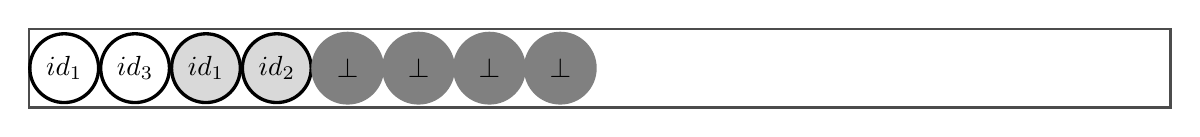
\begin{tikzpicture}
 [
 greenball/.style={circle, draw=black, fill=gray!30, very thick, minimum size=7mm},
 redball/.style={circle, draw=black, fill=white, very thick, minimum size=7mm},
 dummyball/.style={circle, draw=gray, fill=gray, very thick, minimum size=7mm},
 textbox/.style={rectangle, draw=white, fill=white, thick, minimum height=1cm},
 buffer1/.style={rectangle, draw=black!70, fill=white, thick, minimum height=1cm,minimum width=14.5cm}
 ]
  \node at (0,0) [buffer1] (buf) {};
 \node at (-6.8,0) [redball]   (ball1)    {$id_1$};
 \node at (-5.9,0) [redball]   (ball2)                              {$id_3$};
 \node at (-5,0) [greenball]   (ball3)                              {$id_1$};
 \node at (-4.1,0) [greenball]   (ball4)                              {$id_2$};
 \node at (-3.2,0) [dummyball]   (ball5)                              {$~\bot~$};
 \node at (-2.3,0) [dummyball]   (d1)                              {$~\bot~$};
 \node at (-1.4,0) [dummyball]   (d2)                              {$~\bot~$};
 \node at (-0.5,0) [dummyball]   (d3)                              {$~\bot~$};
%\node at (0.3,-1.2) [textbox]      (tb1)                          {$\BUF_1$};
 \end{tikzpicture}
 \captionsetup{justification=justified,font=large}
 \newsubcaption{$\BUF_1$ after oblivious sort w.r.t lexicographic order of keywords.}
 \label{fig:buf1.1}
 \end{subfigure}
 }
 \end{figure*}



 \begin{figure*}[!h]
 \ContinuedFloat
 \centering
%\scalebox{0.6}
{
 \begin{subfigure}[t]{0.8\textwidth}
\centering
   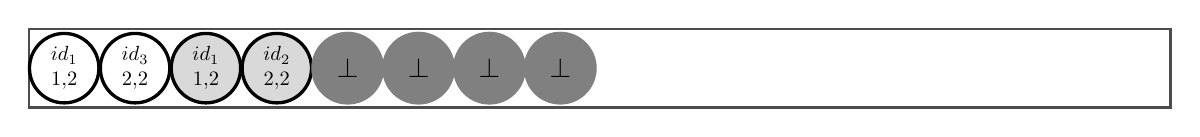
\begin{tikzpicture}
   [
   greenball/.style={circle, draw=black, align=center, fill=gray!30, very thick, minimum size=7mm},
   redball/.style={circle, draw=black,align=center, fill=white, very thick, minimum size=7mm},
   dummyball/.style={circle, draw=gray, align=center, fill=gray, very thick, minimum size=7mm},
   textbox/.style={rectangle, draw=white, fill=white, thick, minimum height=1cm},
   buffer1/.style={rectangle, draw=black!70, fill=white, thick, minimum height=1cm,minimum width=14.5cm},
   ]
 %\node at (0.3,-0.7) [textbox] (tb1) {$\BUF_1$};
 \node at (0,0) [buffer1] (buf) {};
 \node[scale=0.74] at (-6.8,0) [redball]   (ball1)  {$id_1$\\ 1,2};
 \node[scale=0.74] at (-5.9,0) [redball]   (ball2)  {$id_3$\\ 2,2};
 \node[scale=0.74] at (-5,0) [greenball]   (ball3)  {$id_1$\\ 1,2};
 \node[scale=0.74] at (-4.1,0) [greenball]   (ball4) {$id_2$\\ 2,2};
 \node at (-3.2,0) [dummyball]   (ball5)  {$~\bot~$};
 \node at (-2.3,0) [dummyball]   (d1)  {$~\bot~$};
 \node at (-1.4,0) [dummyball]   (d2) {$~\bot~$};
 \node at (-0.5,0) [dummyball]   (d3) {$~\bot~$};
   \end{tikzpicture}
   \captionsetup{justification=centering,font=large}
   \newsubcaption{The first and the second number indicates $rank$ and $n_w$ value respectively. }
   \label{fig:buf1a}
 \end{subfigure}
 }
\end{figure*}


%%%%%%%%%%%%%%%%%%%%%%%%%%%%%THIS ONE
 \begin{figure*}[!h]
 \ContinuedFloat
 \centering
%\scalebox{0.6}
{
 \begin{subfigure}[t]{0.8\textwidth}
\centering
   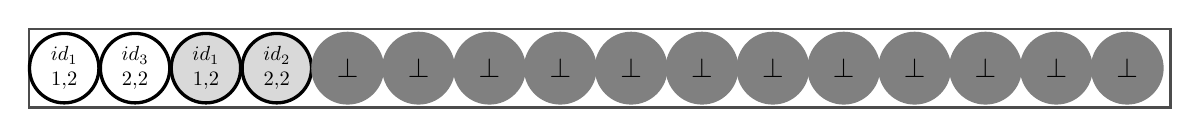
\begin{tikzpicture}
   [
   greenball/.style={circle, draw=black, align=center, fill=gray!30, very thick, minimum size=7mm},
   redball/.style={circle, draw=black,align=center, fill=white, very thick, minimum size=7mm},
   dummyball/.style={circle, draw=gray, align=center, fill=gray, very thick, minimum size=7mm},
   textbox/.style={rectangle, draw=white, fill=white, thick, minimum height=1cm},
   buffer1/.style={rectangle, draw=black!70, fill=white, thick, minimum height=1cm,minimum width=14.5cm},
   ]
 %\node at (0.3,-0.7) [textbox] (tb1) {$\BUF_1$};
 \node at (0,0) [buffer1] (buf) {};
 \node[scale=0.74] at (-6.8,0) [redball]   (ball1)  {$id_1$\\ 1,2};
 \node[scale=0.74] at (-5.9,0) [redball]   (ball2)  {$id_3$\\ 2,2};
 \node[scale=0.74] at (-5,0) [greenball]   (ball3)  {$id_1$\\ 1,2};
 \node[scale=0.74] at (-4.1,0) [greenball]   (ball4) {$id_2$\\ 2,2};
 \node at (-3.2,0) [dummyball]   (ball5)  {$~\bot~$};
 \node at (-2.3,0) [dummyball]   (d1)  {$~\bot~$};
 \node at (-1.4,0) [dummyball]   (d2) {$~\bot~$};
 \node at (-0.5,0) [dummyball]   (d3) {$~\bot~$};
 \node at (0.4,0) [dummyball]   (d4)  {$~\bot~$};
 \node at (1.3,0) [dummyball]   (d5)  {$~\bot~$};
 \node at (2.2,0) [dummyball]   (d6)    {$~\bot~$};
 \node at (3.1,0) [dummyball] (rd7) {$~\bot~$};    
 \node at (4,0) [dummyball]   (d8)   {$~\bot~$};
 \node at (4.9,0) [dummyball]   (d9)   {$~\bot~$};
 \node at (5.8,0) [dummyball]   (d10)   {$~\bot~$};
 \node at (6.7,0) [dummyball]   (d11)   {$~\bot~$};
   \end{tikzpicture}
   \captionsetup{justification=centering,font=large}
   \newsubcaption{$\BUF_1$ after padding each list to power of 2 }
   \label{fig:buf1a}
 \end{subfigure}
 }
%\caption{$\BUF_1$ after different phases}
\end{figure*}

 \begin{figure*}[!h]
 \ContinuedFloat
\centering
 %\scalebox{0.6}
 {
 \begin{subfigure}[t]{0.8\textwidth}
\centering
   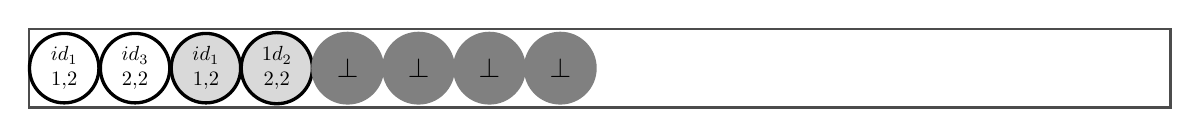
\begin{tikzpicture}
     [
     greenball/.style={circle, draw=black, align=center, fill=gray!30, very thick, minimum size=7mm},
     redball/.style={circle, draw=black,align=center, fill=white, very thick, minimum size=7mm},
     dummyball/.style={circle, draw=gray, align=center, fill=gray, very thick, minimum size=7mm},
     textbox/.style={rectangle, draw=white, fill=white, thick, minimum height=1cm},
     buffer1/.style={rectangle, draw=black!70, fill=white, thick, minimum height=1cm,minimum width=14.5cm},
     ]
  \node at (0,0) [buffer1] (buf) {};
 \node[scale=0.74] at (-6.8,0) [redball]   (ball1)  {$id_1$\\ 1,2};
 \node[scale=0.74] at (-5.9,0) [redball]   (ball2)  {$id_3$\\ 2,2};
 \node[scale=0.74] at (-5,0) [greenball]   (ball5) {$id_1$\\ 1,2};
 \node[scale=0.74] at (-4.1,0) [greenball]   (d1)  {$1d_2$\\ 2,2};
 \node at (-3.2,0) [dummyball]   (d2)  {$~\bot~$};
 \node at (-2.3,0) [dummyball]   (d3)  {$~\bot~$};
 \node at (-1.4,0) [dummyball]   (d2)  {$~\bot~$};
 \node at (-0.5,0) [dummyball]   (d3)  {$~\bot~$};
 \end{tikzpicture}
 \captionsetup{justification=centering,font=large}
 \newsubcaption{$\BUF_1$ at the end of Initialization phase.}
 \label{fig:buf1b}
 \end{subfigure}
 }
 \end{figure*}

 \begin{figure*}[!h]
 \ContinuedFloat
 \centering
 %\scalebox{0.6}
 {
 \begin{subfigure}{0.8\textwidth}
\centering
   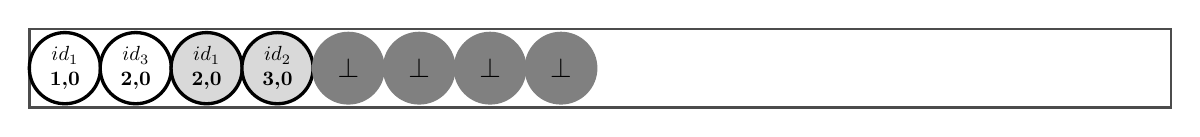
\begin{tikzpicture}
     [
    greenball/.style={circle, draw=black, align=center, fill=gray!30, very thick, minimum size=7mm},
   redball/.style={circle, draw=black,align=center, fill=white, very thick, minimum size=7mm},
     dummyball/.style={circle, draw=gray, align=center, fill=gray, very thick, minimum size=7mm},
     textbox/.style={rectangle, draw=white, fill=white, thick, minimum height=1cm},
     buffer1/.style={rectangle, draw=black!70, fill=white, thick, minimum height=1cm,minimum width=14.5cm},
     ]
  \node at (0,0) [buffer1] (buf) {};
 \node[scale=0.74] at (-6.8,0) [redball]   (ball1)  {$id_1$\\ \tblue{\textbf{1,0}}};
 \node[scale=0.74] at (-5.9,0) [redball]   (ball2)  {$id_3$\\ \tblue{\textbf{2,0}}};
 \node[scale=0.74] at (-5,0) [greenball]   (ball3) {$id_1$\\ \tblue{\textbf{2,0}}};
 \node[scale=0.74] at (-4.1,0) [greenball]   (ball4) {$id_2$\\ \tblue{\textbf{3,0}}};
 \node at (-3.2,0) [dummyball]   (ball5) {$~\bot~$};
 \node at (-2.3,0) [dummyball]   (d1)  {$~\bot~$};
 \node at (-1.4,0) [dummyball]   (d2)  {$~\bot~$};
 \node at (-0.5,0) [dummyball]   (d3)  {$~\bot~$};
%\node at (6.7,0) [dummyball]   (d11)   {$~\bot~$};
   \end{tikzpicture}
   \captionsetup{justification=centering,font=large}
   \newsubcaption{$\BUF_1$ at the end of Phase 1. First number indicates the new bin number. The second number is by default 0 for \OneChoice.}
   \label{fig:buf1c}
 \end{subfigure}
 }
 \end{figure*}

 \begin{figure*}[!h]
 \ContinuedFloat
 \centering
 %\scalebox{0.6}
 {
 \begin{subfigure}[]{0.8\textwidth}
\centering
   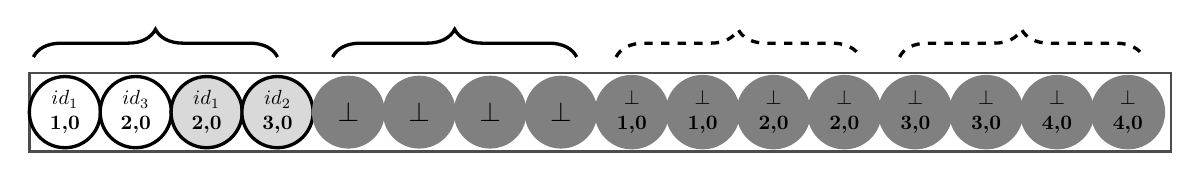
\begin{tikzpicture}
     [
     greenball/.style={circle, draw=black, align=center, fill=gray!30, very thick, minimum size=7mm},
     redball/.style={circle, draw=black,align=center, fill=white, very thick, minimum size=7mm},
     dummyball/.style={circle, draw=gray, align=center, fill=gray, very thick, minimum size=7mm},
     textbox/.style={rectangle, draw=white, fill=white, thick, minimum height=1cm},
     buffer1/.style={rectangle, draw=black!70, fill=white, thick, minimum height=1cm,minimum width=14.5cm},
     ]
  \node at (0,0) [buffer1] (buf) {};
\draw [decorate, decoration = {brace, amplitude = 10pt},very thick] (-7.2,0.7) --  (-4.1,0.7);
\draw [decorate, decoration = {brace, amplitude = 10pt},very thick] (-3.4,0.7) --  (-0.3,0.7);
\draw [decorate, decoration = {brace, amplitude = 10pt},very thick, dashed] (0.2,0.7) --  (3.3,0.7);
\draw [decorate, decoration = {brace, amplitude = 10pt},very thick, dashed] (3.8,0.7) --  (6.9,0.7);
  \node[scale=0.74] at (-6.8,0) [redball]   (ball1)  {$id_1$\\ \tblue{\textbf{1,0}}};
 \node[scale=0.74] at (-5.9,0) [redball]   (ball2)  {$id_3$\\ \tblue{\textbf{2,0}}};
 \node[scale=0.74] at (-5,0) [greenball]   (ball3) {$id_1$\\ \tblue{\textbf{2,0}}};
 \node[scale=0.74] at (-4.1,0) [greenball]   (ball4) {$id_2$\\ \tblue{\textbf{3,0}}};
\node at (-3.2,0) [dummyball]   (ball5) {$~\bot~$};
 \node at (-2.3,0) [dummyball]   (d1)  {$~\bot~$};
 \node at (-1.4,0) [dummyball]   (d2)  {$~\bot~$};
 \node at (-0.5,0) [dummyball]   (d3)  {$~\bot~$};
 \node[scale=0.74] at (0.4,0) [dummyball]   (d4)  {$~\bot~$\\ \tblue{\textbf{1,0}}};
 \node[scale=0.74] at (1.3,0) [dummyball]   (d5)  {$~\bot~$\\ \tblue{\textbf{1,0}}};
 \node[scale=0.74] at (2.2,0) [dummyball]   (d6)  {$~\bot~$\\ \tblue{\textbf{2,0}}};
 \node[scale=0.74] at (3.1,0) [dummyball] (rd7) {$~\bot~$\\ \tblue{\textbf{2,0}}};  
 \node[scale=0.74] at (4,0) [dummyball] (d8) {$~\bot~$\\ \tblue{\textbf{3,0}}};
 \node[scale=0.74] at (4.9,0) [dummyball] (d9) {$~\bot~$\\ \tblue{\textbf{3,0}}};
 \node[scale=0.74] at (5.8,0) [dummyball] (d10)  {$~\bot~$\\ \tblue{\textbf{4,0}}};
 \node[scale=0.74] at (6.7,0) [dummyball]  (d11) {$~\bot~$\\ \tblue{\textbf{4,0}}};
   \end{tikzpicture}
   \captionsetup{justification=centering,font=large}
   \newsubcaption{$\BUF_1$ at the end of Phase 2.Two dummy entries appended for each bin. The braces indicate the bins for the oblivious sort of (next) Phase 3. Two consecutive bucket elements are merged and sorted locally at the client and again written back to two consecutive buckets, as shown in Figure \ref{fig:buf1d} below.}
   \label{fig:buf1d}
 \end{subfigure}
 }
 \end{figure*}

\begin{figure*}[!h]
 \ContinuedFloat
 \centering
 %\scalebox{0.6}
 {
 \begin{subfigure}[]{0.8\textwidth}
\centering
   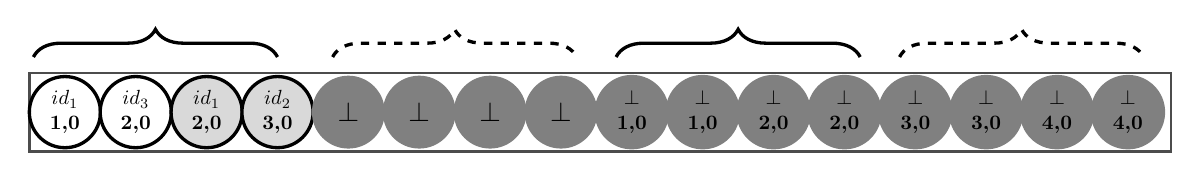
\begin{tikzpicture}
     [
     greenball/.style={circle, draw=black, align=center, fill=gray!30, very thick, minimum size=7mm},
     redball/.style={circle, draw=black,align=center, fill=white, very thick, minimum size=7mm},
     dummyball/.style={circle, draw=gray, align=center, fill=gray, very thick, minimum size=7mm},
     textbox/.style={rectangle, draw=white, fill=white, thick, minimum height=1cm},
     buffer1/.style={rectangle, draw=black!70, fill=white, thick, minimum height=1cm,minimum width=14.5cm},
     ]
  \node at (0,0) [buffer1] (buf) {};
\draw [decorate, decoration = {brace, amplitude = 10pt},very thick] (-7.2,0.7) --  (-4.1,0.7);
\draw [decorate, decoration = {brace, amplitude = 10pt},very thick, dashed] (-3.4,0.7) --  (-0.3,0.7);
\draw [decorate, decoration = {brace, amplitude = 10pt},very thick] (0.2,0.7) --  (3.3,0.7);
\draw [decorate, decoration = {brace, amplitude = 10pt},very thick, dashed] (3.8,0.7) --  (6.9,0.7);
  \node[scale=0.74] at (-6.8,0) [redball]   (ball1)  {$id_1$\\ \tblue{\textbf{1,0}}};
 \node[scale=0.74] at (-5.9,0) [redball]   (ball2)  {$id_3$\\ \tblue{\textbf{2,0}}};
 \node[scale=0.74] at (-5,0) [greenball]   (ball3) {$id_1$\\ \tblue{\textbf{2,0}}};
 \node[scale=0.74] at (-4.1,0) [greenball]   (ball4) {$id_2$\\ \tblue{\textbf{3,0}}};
\node at (-3.2,0) [dummyball]   (ball5) {$~\bot~$};
 \node at (-2.3,0) [dummyball]   (d1)  {$~\bot~$};
 \node at (-1.4,0) [dummyball]   (d2)  {$~\bot~$};
 \node at (-0.5,0) [dummyball]   (d3)  {$~\bot~$};
 \node[scale=0.74] at (0.4,0) [dummyball]   (d4)  {$~\bot~$\\ \tblue{\textbf{1,0}}};
 \node[scale=0.74] at (1.3,0) [dummyball]   (d5)  {$~\bot~$\\ \tblue{\textbf{1,0}}};
 \node[scale=0.74] at (2.2,0) [dummyball]   (d6)  {$~\bot~$\\ \tblue{\textbf{2,0}}};
 \node[scale=0.74] at (3.1,0) [dummyball] (rd7) {$~\bot~$\\ \tblue{\textbf{2,0}}};  
 \node[scale=0.74] at (4,0) [dummyball] (d8) {$~\bot~$\\ \tblue{\textbf{3,0}}};
 \node[scale=0.74] at (4.9,0) [dummyball] (d9) {$~\bot~$\\ \tblue{\textbf{3,0}}};
 \node[scale=0.74] at (5.8,0) [dummyball] (d10)  {$~\bot~$\\ \tblue{\textbf{4,0}}};
 \node[scale=0.74] at (6.7,0) [dummyball]  (d11) {$~\bot~$\\ \tblue{\textbf{4,0}}};
   \end{tikzpicture}
   \captionsetup{justification=centering,font=large}
   \newsubcaption{$\BUF_1$ at an intermediate state during the oblivious merge of Phase 3. This is the output after one of the  calls (out of $2^i$ calls) to \omerge$_i$. Next, two alternative bucket elements are merged and sorted locally, and again written back to two consecutive buckets, as shown in Figure \ref{fig:buf1e} below.}
   \label{fig:buf1d}
 \end{subfigure}
 }
 \end{figure*}




 \begin{figure*}[!h]
 \ContinuedFloat
 \centering
 %\scalebox{0.6}
 {
 \begin{subfigure}[]{0.8\textwidth}
 \centering
   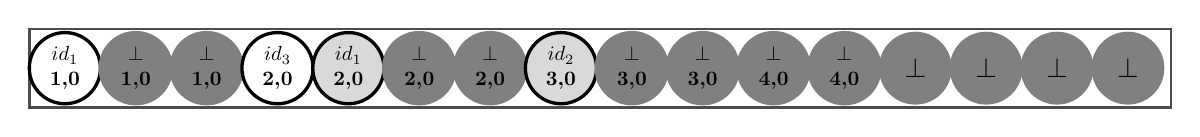
\begin{tikzpicture}
     [
     greenball/.style={circle, draw=black, align=center, fill=gray!30, very thick, minimum size=7mm},
     redball/.style={circle, draw=black,align=center, fill=white, very thick, minimum size=7mm},
     dummyball/.style={circle, draw=gray, align=center, fill=gray, very thick, minimum size=7mm},
     textbox/.style={rectangle, draw=white, fill=white, thick, minimum height=1cm},
     buffer1/.style={rectangle, draw=black!70, fill=white, thick, minimum height=1cm,minimum width=14.5cm},
     ]
  \node at (0,0) [buffer1] (buf) {};
 % \draw [decorate, decoration = {brace, amplitude = 10pt},very thick] (-7.2,0.7) --  (-4.1,0.7);
%\draw [decorate, decoration = {brace, amplitude = 10pt},very thick] (-3.4,0.7) --  (-0.3,0.7);
%\draw [decorate, decoration = {brace, amplitude = 10pt},very thick] (0.2,0.7) --  (3.3,0.7);
%\draw [decorate, decoration = {brace, amplitude = 10pt},very thick] (3.8,0.7) --  (6.9,0.7);
 \node[scale=0.74] at (-6.8,0) [redball]   (ball1)  {$id_1$\\ \tblue{\textbf{1,0}}};
 \node[scale=0.74] at (-5.9,0) [dummyball]   (ball2)  {$~\bot~$\\ \tblue{\textbf{1,0}}};
 \node[scale=0.74] at (-5,0) [dummyball]   (ball3) {$~\bot~$\\ \tblue{\textbf{1,0}}};
 \node[scale=0.74] at (-4.1,0) [redball]   (ball4) {$id_3$\\ \tblue{\textbf{2,0}}};
 \node[scale=0.74] at (-3.2,0) [greenball]   (ball5) {$id_1$\\ \tblue{\textbf{2,0}}};
 \node[scale=0.74] at (-2.3,0) [dummyball]   (d1)  {$~\bot~$\\ \tblue{\textbf{2,0}}};
 \node[scale=0.74] at (-1.4,0) [dummyball]   (d2)  {$~\bot~$\\ \tblue{\textbf{2,0}}};
 \node[scale=0.74] at (-0.5,0) [greenball]   (d3)  {$id_2$\\ \tblue{\textbf{3,0}}};
 \node[scale=0.74] at (0.4,0) [dummyball]   (d4)  {$~\bot~$\\ \tblue{\textbf{3,0}}};
 \node[scale=0.74] at (1.3,0) [dummyball]   (d5)  {$~\bot~$\\ \tblue{\textbf{3,0}}};
 
 \node[scale=0.74] at (2.2,0) [dummyball]   (d6)  {$~\bot~$\\ \tblue{\textbf{4,0}}};
 \node[scale=0.74] at (3.1,0) [dummyball] (rd7) {$~\bot~$\\ \tblue{\textbf{4,0}}};    
 \node at (4,0) [dummyball] (d8) {$~\bot~$};
 \node at (4.9,0) [dummyball] (d9) {$~\bot~$};
 \node at (5.8,0) [dummyball] (d10)  {$~\bot~$};
 \node at (6.7,0) [dummyball]  (d11) {$~\bot~$};
   \end{tikzpicture}
   \captionsetup{justification=centering,font=large}
   \newsubcaption{$\BUF_1$ after the oblivious sort in Phase 3. This is just the state of $\BUF_1$ at the end of Phase 3, but the \omerge\ call may not be done yet. Recall that one call of \omerge\ performs a $\gamma$ number of steps. Those $\gamma$ number of steps may distribute across phases as well. The phases are created only for representation purpose.
   }
   \label{fig:buf1e}
 \end{subfigure}
 }
 \end{figure*}




 \begin{figure*}[!h]
 \ContinuedFloat
 \centering
 %\scalebox{0.6}
 {
 \begin{subfigure}[]{0.8\textwidth}
 \centering
   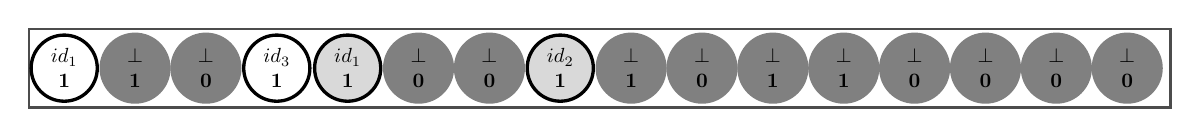
\begin{tikzpicture}
     [
     greenball/.style={circle, draw=black, align=center, fill=gray!30, very thick, minimum size=7mm},
     redball/.style={circle, draw=black,align=center, fill=white, very thick, minimum size=7mm},
     dummyball/.style={circle, draw=gray, align=center, fill=gray, very thick, minimum size=7mm},
     textbox/.style={rectangle, draw=white, fill=white, thick, minimum height=1cm},
     buffer1/.style={rectangle, draw=black!70, fill=white, thick, minimum height=1cm,minimum width=14.5cm},
     ]
  \node at (0,0) [buffer1] (buf) {};
 \node[scale=0.74] at (-6.8,0) [redball]   (ball1)  {$id_1$\\ \tblue{\textbf{1}}};
 \node[scale=0.74] at (-5.9,0) [dummyball]   (ball2)  {$~\bot~$\\ \tblue{\textbf{1}}};
 \node[scale=0.74] at (-5,0) [dummyball]   (ball3) {$~\bot~$\\ \tred{\textbf{0}}};
 \node[scale=0.74] at (-4.1,0) [redball]   (ball4) {$id_3$\\ \tblue{\textbf{1}}};
 \node[scale=0.74] at (-3.2,0) [greenball]   (ball5) {$id_1$\\ \tblue{\textbf{1}}};
 \node[scale=0.74] at (-2.3,0) [dummyball]   (d1)  {$~\bot~$\\ \tred{\textbf{0}}};
 \node[scale=0.74] at (-1.4,0) [dummyball]   (d2)  {$~\bot~$\\ \tred{\textbf{0}}};
 \node[scale=0.74] at (-0.5,0) [greenball]   (d3)  {$id_2$\\ \tblue{\textbf{1}}};
 \node[scale=0.74] at (0.4,0) [dummyball]   (d4)  {$~\bot~$\\ \tblue{\textbf{1}}};
 \node[scale=0.74] at (1.3,0) [dummyball]   (d5)  {$~\bot~$\\ \tred{\textbf{0}}};
 \node[scale=0.74] at (2.2,0) [dummyball]   (d6)  {$~\bot~$\\ \tblue{\textbf{1}}};
 \node[scale=0.74] at (3.1,0) [dummyball] (rd7) {$~\bot~$\\ \tblue{\textbf{1}}};    
 \node[scale=0.74] at (4,0) [dummyball] (d8) {$~\bot~$\\ \tred{\textbf{0}}};
 \node[scale=0.74] at (4.9,0) [dummyball] (d9) {$~\bot~$\\ \tred{\textbf{0}}};
 \node[scale=0.74] at (5.8,0) [dummyball] (d10)  {$~\bot~$\\ \tred{\textbf{0}}};
 \node[scale=0.74] at (6.7,0) [dummyball]  (d11) {$~\bot~$\\ \tred{\textbf{0}}};
   \end{tikzpicture}
   \captionsetup{justification=centering,font=large}
   \newsubcaption{$\BUF_1$ after the linear scan and adding 1/0-bit tag in Phase 3}
   \label{fig:buf1f}
 \end{subfigure}
 }
 \end{figure*}

 \begin{figure*}[!h]
 \ContinuedFloat
 \centering
 %\scalebox{0.6}
 {
 \begin{subfigure}[]{0.8\textwidth}
 \centering
   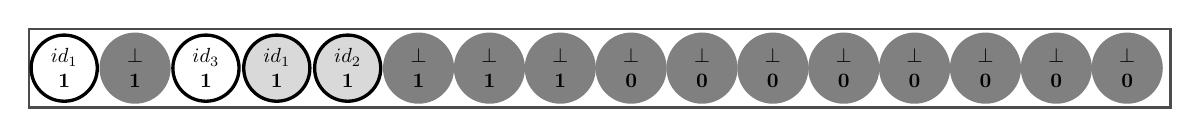
\begin{tikzpicture}
     [
     greenball/.style={circle, draw=black, align=center, fill=gray!30, very thick, minimum size=7mm},
     redball/.style={circle, draw=black,align=center, fill=white, very thick, minimum size=7mm},
     dummyball/.style={circle, draw=gray, align=center, fill=gray, very thick, minimum size=7mm},
     textbox/.style={rectangle, draw=white, fill=white, thick, minimum height=1cm},
     buffer1/.style={rectangle, draw=black!70, fill=white, thick, minimum height=1cm,minimum width=14.5cm},
     ]
  \node at (0,0) [buffer1] (buf) {};
 \node[scale=0.74] at (-6.8,0) [redball]   (ball1)  {$id_1$\\ \tblue{\textbf{1}}};
 \node[scale=0.74] at (-5.9,0) [dummyball]   (ball2)  {$~\bot~$\\ \tblue{\textbf{1}}};
 \node[scale=0.74] at (-5,0) [redball]   (ball3) {$id_3$\\ \tblue{\textbf{1}}};
 \node[scale=0.74] at (-4.1,0) [greenball]   (ball4) {$id_1$\\ \tblue{\textbf{1}}};
 \node[scale=0.74] at (-3.2,0) [greenball]   (ball5) {$id_2$\\ \tblue{\textbf{1}}};
 \node[scale=0.74] at (-2.3,0) [dummyball]   (d1)  {$~\bot~$\\ \tblue{\textbf{1}}};
 \node[scale=0.74] at (-1.4,0) [dummyball]   (d2)  {$~\bot~$\\ \tblue{\textbf{1}}};
 \node[scale=0.74] at (-0.5,0) [dummyball]   (d3)  {$~\bot~$\\ \tblue{\textbf{1}}};
 \node[scale=0.74] at (0.4,0) [dummyball]   (d4)  {$~\bot~$\\ \tred{\textbf{0}}};
 \node[scale=0.74] at (1.3,0) [dummyball]   (d5)  {$~\bot~$\\ \tred{\textbf{0}}};
 \node[scale=0.74] at (2.2,0) [dummyball]   (d6)  {$~\bot~$\\ \tred{\textbf{0}}};
 \node[scale=0.74] at (3.1,0) [dummyball] (rd7) {$~\bot~$\\ \tred{\textbf{0}}};    
 \node[scale=0.74] at (4,0) [dummyball] (d8) {$~\bot~$\\ \tred{\textbf{0}}};
 \node[scale=0.74] at (4.9,0) [dummyball] (d9) {$~\bot~$\\ \tred{\textbf{0}}};
 \node[scale=0.74] at (5.8,0) [dummyball] (d10)  {$~\bot~$\\ \tred{\textbf{0}}};
 \node[scale=0.74] at (6.7,0) [dummyball]  (d11) {$~\bot~$\\ \tred{\textbf{0}}};
   \end{tikzpicture}
   \captionsetup{justification=centering,font=large}
   \newsubcaption{$\BUF_1$ after the order preserving oblivious compaction in Phase 3}
 \label{fig:buf1g}
 \end{subfigure}
 }
 \end{figure*}


 \begin{figure*}[!h]
 \ContinuedFloat
 \centering
 %\scalebox{0.6}
 {
 \begin{subfigure}[]{0.8\textwidth}
 \centering
   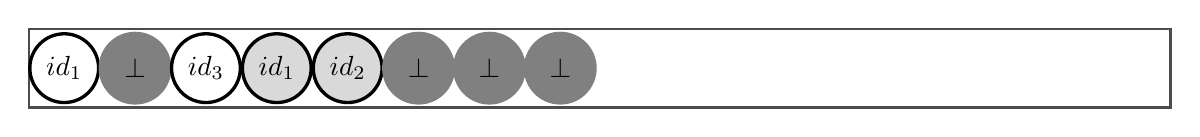
\begin{tikzpicture}
     [
     greenball/.style={circle, draw=black, align=center, fill=gray!30, very thick, minimum size=7mm},
     redball/.style={circle, draw=black,align=center, fill=white, very thick, minimum size=7mm},
     dummyball/.style={circle, draw=gray, align=center, fill=gray, very thick, minimum size=7mm},
     textbox/.style={rectangle, draw=white, fill=white, thick, minimum height=1cm},
     buffer1/.style={rectangle, draw=black!70, fill=white, thick, minimum height=1cm,minimum width=14.5cm},
     ]
  \node at (0,0) [buffer1] (buf) {};
 \node at (-6.8,0) [redball]   (ball1)  {$id_1$};
 \node[scale=1] at (-5.9,0) [dummyball]   (ball2)  {$~\bot~$};
 \node[scale=1] at (-5,0) [redball]   (ball3) {$id_3$};
 \node[scale=1] at (-4.1,0) [greenball]   (ball4) {$id_1$};
 \node[scale=1] at (-3.2,0) [greenball]   (ball5) {$id_2$};
 \node[scale=1] at (-2.3,0) [dummyball]   (d1)  {$~\bot~$};
 \node[scale=1] at (-1.4,0) [dummyball]   (d2)  {$~\bot~$};
 \node at (-0.5,0) [dummyball]   (d3)  {$~\bot~$};
 \end{tikzpicture}
   \captionsetup{justification=centering,font=large}
   \newsubcaption{$\BUF_1$ after discarding the 0/1-bit tags; at the end of Phase 3}
   \label{fig:buf1h}
 \end{subfigure}
 }
 \end{figure*}


%Every $b_i$ elements are randomly shuffled.


 \begin{figure*}[!h]
 \ContinuedFloat
 \centering
 %\scalebox{0.6}{
 \begin{subfigure}[]{0.5\textwidth}
 \centering
     \begin{tikzpicture}
 [
 greenball/.style={circle, draw=black, align=center, fill=gray!30, very thick, minimum size=7mm},
 redball/.style={circle, draw=black,align=center, fill=white, very thick, minimum size=7mm},
 blueball/.style={circle, draw=blue!40, fill=blue!40, very thick, minimum size=7mm},
 yellowball/.style={circle, draw=yellow!40, fill=yellow!40, very thick, minimum size=7mm},
 dummyball/.style={circle, draw=gray, fill=gray, very thick, minimum size=7mm},
 bin/.style={cylinder, draw=black!70, fill=white, thick, minimum height=2.4cm, minimum width = 1cm, rotate=90},
 textbox/.style={rectangle, draw=white, fill=white, thick, minimum height=1cm}
 ]
  \node at (1,0.5) [bin] (bin1) {};
 \node at (1,0) [redball]  (ball1)  {$id_1$};
 \node at (1,1) [dummyball]   (d1)  {$~\bot~$};
 \node at (2.3,0.5) [bin] (bin2) {};
 \node at (2.3,0) [greenball]   (d2)  {$id_1$};
 \node at (2.3,1) [redball]  (ball2) {$id_3$};
 \node at (3.6,0.5) [bin] (bin1) {};
 \node at (3.6,0) [dummyball]      (ball3)    {$~\bot~$};
 \node at (3.6,1) [greenball]      (d3)    {$id_2$};
 \node at (4.9,0.5) [bin] (bin2) {};
  \node at (4.9,0) [dummyball]      (ball4)  {$~\bot~$};
  \node at (4.9,1) [redball]      (ball5)    {$~\bot~$};
 \end{tikzpicture}
 \captionsetup{justification=centering,font=large}
 \newsubcaption{$\NEW_{i}.\Ind$ after random shuffle}
 \label{fig:buf1i}
 \end{subfigure}
 %}
 \caption{Different phases and steps of \omerge. Figure \ref{fig:buf1d} shows an an intermediate $\BUF_1$ state after a call to \omerge$_i$. The whole process takes a total of $2^i$ calls to \omerge$_i$. We have only shown the index part, and omitted the dictionary.}
 \label{fig:LSDdEx}
 \end{figure*}






\section{Performance of Amortized Schemes} \label{append:perf-amort}

In this section, we evaluate the performance of the amortized schemes and provide some experiments for their real-world use case. 

Figure~\ref{app-fig:update} shows an experiment that  measures the update time for 1K consecutive updates. In each update, the client fetches and merges some of the previously built levels and then uploads them to the server. 

Figure~\ref{app-fig:real} shows the search for different result sizes on two attributes of the crime dataset \cite{crimes}, each of which has (a) $34$, (b) $170$ distinct keywords. We measured the search time for different keywords associated with  the increasing number of results.

Figure~\ref{app-fig:search-var-amor-deamor} shows the search  time of different amortized schemes (including \LSDd[$sN$] for $s$ equal to 3 and 6) for a dataset with size $2^{23}$ when the result size varies between 10 and 5M.

Figure~\ref{app-fig:search-var} compares different amortized schemes in HDD (a,b,c,d) and SSD (e,f,g) for variable result sizes (a,b,e) and variable dataset sizes (c,d,f,g). All figures except Figure~\ref{app-fig:search-var}(b) which shows the result for block size 512, represent the experiment results for $|block|=32$.

\begin{figure}[!ht]
	\centering
	\begin{subfigure}[t]{0.48\linewidth}
		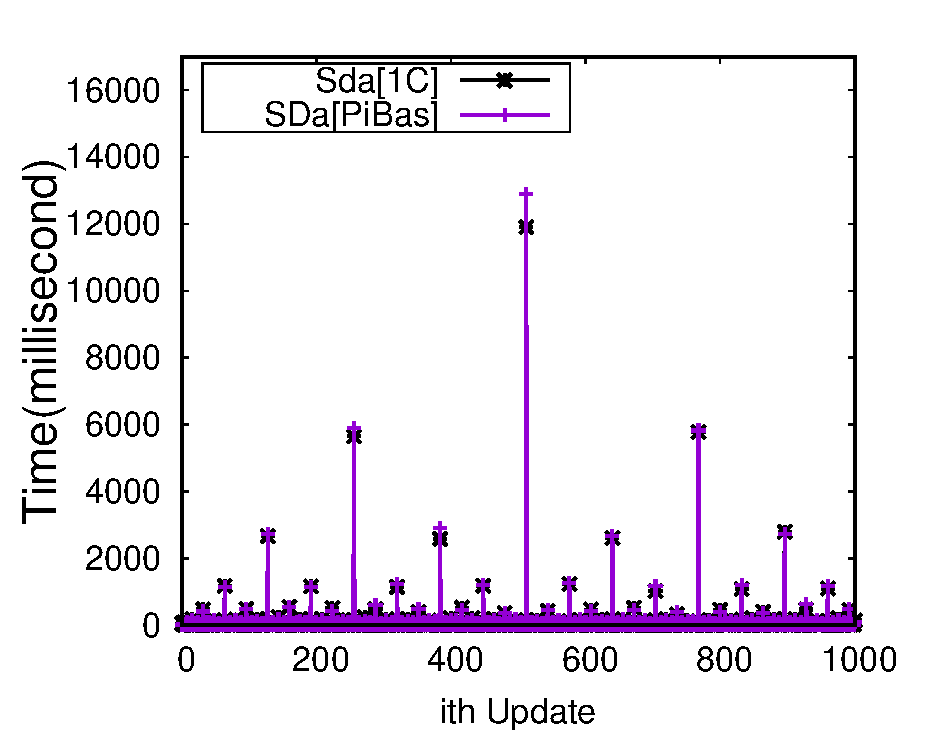
\includegraphics[width=\textwidth]{chapters/iodse/figures/Insert-SDA2.eps}
		\vspace{-0.6cm}
		\caption{}
	\end{subfigure}
 \begin{subfigure}[t]{0.48\linewidth}
		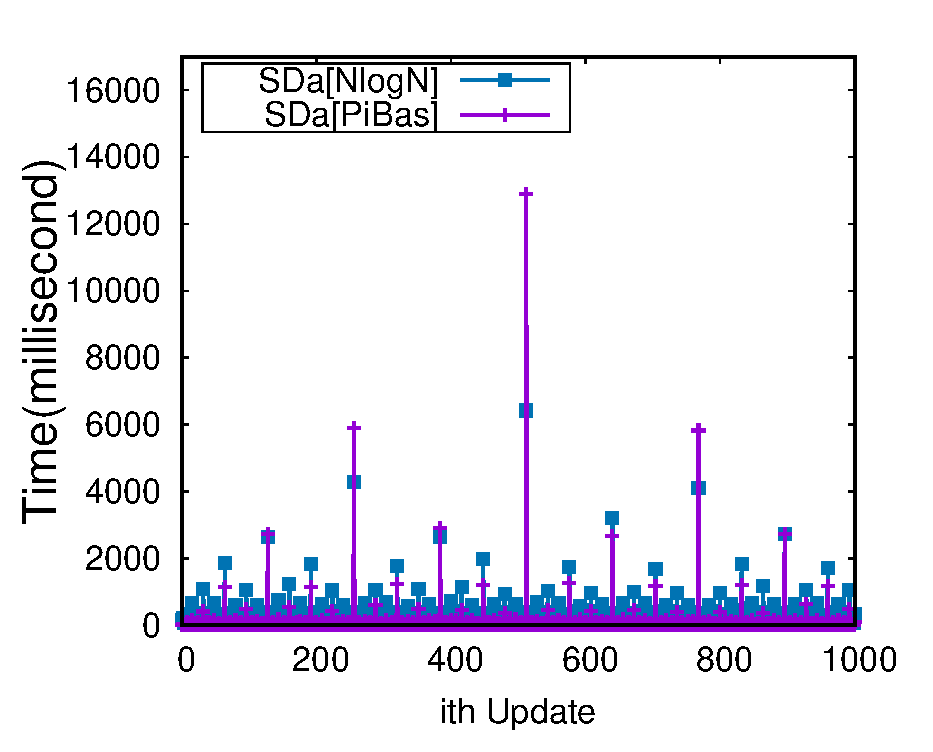
\includegraphics[width=\textwidth]{chapters/iodse/figures/Insert-SDA3.eps}
		\vspace{-0.6cm}
		\caption{}
	\end{subfigure}
	\vspace{-.3cm}
	\caption{Update computation time of amortized schemes for 1K updates starting from an empty dataset (a) \SDa[\OneChoice] vs \SDa[\PiBas] (b) \SDa[\NlogN] vs \SDa[\PiBas] }
	\label{app-fig:update}
% 	\vspace{-.3cm}
\end{figure}


\begin{figure}[!ht]
	\centering
	\begin{subfigure}[t]{0.48\linewidth}
		\includegraphics[width=\textwidth]{chapters/iodse/figures/Search-Crime1.eps}
		\vspace{-0.8cm}
		\caption{}
	\end{subfigure}
	\begin{subfigure}[t]{0.48\linewidth}
		\includegraphics[width=\textwidth]{chapters/iodse/figures/Search-Crime2.eps}
		\vspace{-.8cm}
		\caption{}
	\end{subfigure}%
	
	\vspace{-.3cm}
	\caption{Crime Dataset---Search computation time vs variable result size for an attributed with (a) $|W|=34$, (b) $|W|=170$.}
	\label{app-fig:real}
% 	\vspace{-.3cm}
\end{figure}





\begin{figure}[!ht]
	\centering
	\begin{subfigure}[t]{0.49\linewidth}
		\includegraphics[width=\textwidth]{chapters/iodse/figures/Search-SDA.eps}
		\vspace{-0.8cm}
		\caption{}
	\end{subfigure}
	\begin{subfigure}[t]{0.49\linewidth}
		\includegraphics[width=\textwidth]{chapters/iodse/figures/Search-SDA-SSD.eps}
		\vspace{-.8cm}
		\caption{}
	\end{subfigure}%
	\vspace{-.3cm}
	\caption{Search computation time for $|{DB}|=2^{23}$, variable result size, and $|block|=32$B for different \NlogN settings in (a) amortized HDD, (b) amortized SSD.}
	\label{app-fig:search-var-amor-deamor}
% 	\vspace{-.3cm}
\end{figure}


\begin{figure*}[ht]
	\centering
	\begin{subfigure}[t]{0.24\linewidth}
		\includegraphics[width=\textwidth]{chapters/iodse/figures/Search-Comp-DBSize10M-ResultSizeVar-32B-NoCache-2.eps}
		\vspace{-0.8cm}
		\caption{}
	\end{subfigure}
	\begin{subfigure}[t]{0.24\linewidth}
		\includegraphics[width=\textwidth]{chapters/iodse/figures/Search-Comp-DBSize10M-ResultSizeVar-512B-NoCache-2.eps}
		\vspace{-.8cm}
		\caption{}
	\end{subfigure}%
		\begin{subfigure}[t]{0.24\linewidth}
		\includegraphics[width=\textwidth]{chapters/iodse/figures/Search-Comp-DBSizeVar-ResultSize1000-2.eps}
		\vspace{-.8cm}
		\caption{}
	\end{subfigure}~
 	\begin{subfigure}[t]{0.24\linewidth}
		\includegraphics[width=\textwidth]{chapters/iodse/figures/Search-Comp-DBSizeVar-ResultSize10000-2.eps}
		\vspace{-.8cm}
		\caption{}
	\end{subfigure}~\\
% 	\vspace{-.4cm}
% 	\caption{Search computation time for $|{DB}|=2^{23}$ and variable result size for: (a) $|block|=32$B in HDD, (a) $|block|=32$B in SSD, (c) $|block|=512$B in HDD.}
% 	\label{fig:search-var-block}
	\vspace{-.2cm}
% \end{figure*}

% \begin{figure*}[ht]
% 	\centering
	\begin{subfigure}[t]{0.24\linewidth}
		\includegraphics[width=\textwidth]{chapters/iodse/figures/Search-Comp-DBSize10M-ResultSizeVar-32B-NoCache-SSD-2.eps}
		\vspace{-0.8cm}
		\caption{}
	\end{subfigure}
	\begin{subfigure}[t]{0.24\linewidth}
		\includegraphics[width=\textwidth]{chapters/iodse/figures/Search-Comp-DBSizeVar-ResultSize1000-SSD-2.eps}
		\vspace{-.8cm}
		\caption{}
	\end{subfigure}%
		\begin{subfigure}[t]{0.24\linewidth}
		\includegraphics[width=\textwidth]{chapters/iodse/figures/Search-Comp-DBSizeVar-ResultSize10000-SSD-2.eps}
		\vspace{-.8cm}
		\caption{}
	\end{subfigure}~
	\vspace{-.3cm}
	\caption{Search computation time for $|{DB}|=2^{23}$ and variable result size for (a) $|block|=32$B in HDD, (b) $|block|=512$B in HDD. Search computation time for variable database size and (c) $n_w=1K$ in HDD, (d) $n_w=10K$ in HDD. Search computation time for $|{DB}|=2^{23}$ and variable result size for (e) $|block|=32$B in SSD. Search computation time for variable database size and (f) $n_w=1K$ in SSD, (g) $n_w=10K$ in SSD.}
	\label{app-fig:search-var}
% 	\vspace{-.3cm}
\end{figure*}


\section{Performance of De-Amortized Schemes} \label{append:perf-deamort}

In this section, we provide some extra experiments for the de-amortized schemes. Figure~\ref{app-fig:search-var2} (a) shows the search time when the result size varies between 10 and 5M where the dataset size is $2^{23}$ and the block size is $512$ bytes. Figure~\ref{app-fig:search-var2} (b,c) show the search computation time where database size varies between $2^{14}-2^{26}$ for (b) HDD and (c) SSD. Finally, Figure~\ref{app-fig:search-var2} (d) shows the end-to-end search time over WAN where the machines are located in Ireland and Frankfurt with 24.7ms delay.

\begin{figure*}[ht]
	\centering
	\begin{subfigure}[t]{0.24\linewidth}
		\includegraphics[width=\textwidth]{chapters/iodse/figures/Cache-25-SSD.eps}
		\vspace{-.8cm}
		\caption{}
	\end{subfigure}%
		\begin{subfigure}[t]{0.24\linewidth}
		\includegraphics[width=\textwidth]{chapters/iodse/figures/Cache-50-SSD.eps}
		\vspace{-.8cm}
		\caption{}
	\end{subfigure}~
 	\begin{subfigure}[t]{0.24\linewidth}
		\includegraphics[width=\textwidth]{chapters/iodse/figures/Cache-75-SSD.eps}
		\vspace{-.8cm}
		\caption{}
	\end{subfigure}
    \begin{subfigure}[t]{0.24\linewidth}
		\includegraphics[width=\textwidth]{chapters/iodse/figures/Cache-100.eps}
		\vspace{-0.8cm}
		\caption{}
	\end{subfigure}~\\
	\vspace{-.4cm}
	\caption{Search computation time for $|{DB}|=2^{23}$ and variable result size for $|block|=32$B in SSD, (a) 25\% Caching, (b) 50\% Caching, (c) 75\% Caching, (d) 100\% Caching.}
	\label{fig:cache-ssd}
	\vspace{-.2cm}
\end{figure*}

\begin{figure}[ht]
	\centering
	\begin{subfigure}[t]{0.48\linewidth}
		\includegraphics[width=\textwidth]{chapters/iodse/figures/email-hdd.eps}
		\vspace{-0.6cm}
		\caption{}
	\end{subfigure}
 \begin{subfigure}[t]{0.48\linewidth}
		\includegraphics[width=\textwidth]{chapters/iodse/figures/email-ssd.eps}
		\vspace{-0.6cm}
		\caption{}
	\end{subfigure}
	\vspace{-.3cm}
	\caption{Search computation time for $|{DB}|=2^{20}$ for each user and variable result size for $|block|=32$B with caching enabled in (a) HDD where 200 users exist in the system (b) SSD where 75 users exist in the system}
	\label{fig:email}
% 	\vspace{-.3cm}
\end{figure}


\begin{figure}[ht]
	\centering
 \begin{subfigure}[t]{0.48\linewidth}
		\includegraphics[width=\textwidth]{chapters/iodse/figures/UpdateTime.eps}
		\vspace{-0.6cm}
		\caption{}
	\end{subfigure}
 \begin{subfigure}[t]{0.48\linewidth}
		\includegraphics[width=\textwidth]{chapters/iodse/figures/UpdateTime-WAN1.eps}
		\vspace{-0.6cm}
		\caption{}
	\end{subfigure}
	\vspace{-.3cm}	
	\caption{Update computation time for variable database sizes (a) over single machine (b) over WAN machines with 24.7ms network delay and 2.5Gbps bandwidth.}
	\label{fig:wan}
% 	\vspace{-.3cm}
\end{figure}



\begin{figure}
\small
 \centering\begin{tabular}{|c|c|c|} 
\hline
Scheme & Size(GB) for $|DB|=2^{23}$ & Size(GB) for $|DB|=2^{26}$ \\ 
\hline 
 \LSDd[\NlogN] & 49 & 436 \\
 \LSDd[\OneChoice] & 7.5 & 60\\
 \SDd[\PiBas] & 5 & 40 \\
\hline
\end{tabular}
%\end{adjustbox}
\caption{Needed storage for a dataset and encrypted index=$32B$}
\label{table:storage}
\end{figure} 

% \begin{figure}[ht]
% 	\centering

% 	\vspace{-.3cm}	
% 	\caption{Search computation time for $|{DB}|=2^{23}$, $|block|=32$B in HDD and variable result size for WAN machines with 24.7ms network delay and 2.5Gbps bandwidth.}
% 	\label{fig:app-wan}
% % 	\vspace{-.3cm}
% \end{figure}


\begin{figure*}[ht]
	\centering
	\begin{subfigure}[t]{0.24\linewidth}
		\includegraphics[width=\textwidth]{chapters/iodse/figures/Search-Comp-DBSize10M-ResultSizeVar-512B-NoCache.eps}
		\vspace{-.8cm}
		\caption{}
	\end{subfigure}%
 	\begin{subfigure}[t]{0.24\linewidth}
		\includegraphics[width=\textwidth]{chapters/iodse/figures/Search-Comp-DBSizeVar-ResultSize10000.eps}
		\vspace{-.8cm}
		\caption{}
	\end{subfigure}~
		\begin{subfigure}[t]{0.24\linewidth}
		\includegraphics[width=\textwidth]{chapters/iodse/figures/Search-Comp-DBSizeVar-ResultSize10000-SSD.eps}
		\vspace{-.8cm}
		\caption{}
	\end{subfigure}~
  \begin{subfigure}[t]{0.24\linewidth}
		\includegraphics[width=\textwidth]{chapters/iodse/figures/SearchTime-WAN2.eps}
		\vspace{-0.6cm}
	\end{subfigure}\\
	\vspace{-.3cm}
	\caption{Search computation time for $|{DB}|=2^{23}$ and variable result size for (a)  $|block|=512$B in HDD. Search computation time for variable database size and $n_w=10K$ in (b) HDD, (c) SSD. (d) Search computation time for $|{DB}|=2^{23}$, $|block|=32$B in HDD and variable result size for WAN machines with 24.7ms network delay and 2.5Gbps bandwidth..}
	\label{app-fig:search-var2}
% 	\vspace{-.3cm}
\end{figure*}



% \begin{figure*}[ht]
% 	\centering
% 	\begin{subfigure}[t]{0.24\linewidth}
% 		\includegraphics[width=\textwidth]{figures/Search-SDA.eps}
% 		\vspace{-0.8cm}
% 		\caption{}
% 	\end{subfigure}
% 	\begin{subfigure}[t]{0.24\linewidth}
% 		\includegraphics[width=\textwidth]{figures/Search-SDA-SSD.eps}
% 		\vspace{-.8cm}
% 		\caption{}
% 	\end{subfigure}%
% 		\begin{subfigure}[t]{0.24\linewidth}
% 		\includegraphics[width=\textwidth]{figures/Search-SDD.eps}
% 		\vspace{-.8cm}
% 		\caption{}
% 	\end{subfigure}~
% 	\begin{subfigure}[t]{0.24\linewidth}
% 		\includegraphics[width=\textwidth]{figures/Search-SDD-SSD.eps}
% 		\vspace{-.8cm}
% 		\caption{}
% 	\end{subfigure}%
% 	\vspace{-.3cm}
% 	\caption{Search computation time for $|{DB}|=2^{23}$, variable result size, and $|block|=32$B for different \NlogN settings in (a) amortized HDD, (b) amortized SSD, (c) de-amortized HDD, (d) de-Amortized SSD.}
% 	\label{fig:search-var-amor-deamor}
% % 	\vspace{-.3cm}
% \end{figure*}




% \begin{figure}[ht]
% 	\centering
%  \begin{subfigure}[t]{0.48\linewidth}
% 		\includegraphics[width=\textwidth]{figures/Cache-100.eps}
% 		\vspace{-0.6cm}
% 		\caption{}
% 	\end{subfigure}
%  \begin{subfigure}[t]{0.48\linewidth}
% 		\includegraphics[width=\textwidth]{figures/Cache-100-Server.eps}
% 		\vspace{-0.6cm}
% 		\caption{}
% 	\end{subfigure}
% 	\vspace{-.3cm}	
% 	\caption{(a) Search computation time for $|{DB}|=2^{23}$ and variable result size for $|block|=32$B in 100\% Caching (a) the whole search time (b) server time}
% 	\label{fig:cache2}
% % 	\vspace{-.3cm}
% \end{figure}





\begin{figure*}
\centering
\subfloat[1C]
{
\scalebox{0.8}
{
\begin{tikzpicture}
[
greenball/.style={circle, draw=gray, fill=gray,  thick, minimum size=7mm},
redball/.style={circle, draw=gray, fill=white,  thick, minimum size=7mm},
blueball/.style={circle, draw=black, fill=black,  thick, minimum size=7mm},
whiteball/.style={circle, draw=white, fill=white, very thick, minimum size=7mm},
dummyball/.style={circle, draw=gray, fill=gray, very thick, minimum size=7mm},
bin/.style={cylinder, draw=black!70, fill=white, thick, minimum height=2.4cm, minimum width = 1cm, rotate=90},
textbox/.style={rectangle, draw=white, fill=white, thick, minimum height=1cm},
myarrow1/.style={single arrow, draw=blue, fill=green, 
      minimum width = 10pt, single arrow head extend=3pt,
      minimum height=10mm}
]
\node at (2.3,-1) [textbox]      (tb1)    {Index};
 \node at (1,0.5) [bin] (bin1) {};
\node at (1,0) [greenball]      (ball1)    {};
\node at (1,1) [blueball]      (d1)     {};
 \node at (2.3,0.5) [bin] (bin2) {};
 \node at (2.3,0) [blueball]      (d2)    {};
 \node at (2.3,1) [redball]      (ball2)    {};
 \node at (3.6,0.5) [bin] (bin2) {};
 \node at (3.6,0) [blueball]      (d2)    {};
 \node at (3.6,1) [redball]      (ball2)      {};
 
 \draw[] (4.7,1.2) rectangle (6,-0.4) {};
 \node at (5.4,-1) [textbox]      (d1)       {Dictionary};
 \node[scale=0.6] at (5,0.9) [blueball]   (d1)  {};
 \node[scale=0.7] at (5.7,0.9) [whiteball]   (d1)  {3};
 
  \node[scale=0.6] at (5,0.4) [greenball]   (d1)  {};
  \node[scale=0.7] at (5.7,0.4) [whiteball]   (d1)  {1};
  
   \node[scale=0.6] at (5,-0.1) [redball]   (d1)  {};
   \node[scale=0.7] at (5.7,-0.1) [whiteball]   (d1)  {2};
   \draw[] (4.7,0.65) -- (6,0.65) ;
    \draw[] (4.7,0.15) -- (6,0.15) ;
    \draw[thick,dashed] (5.4,1.2) -- (5.4,-0.4) {};
\end{tikzpicture}
}
}
%\hspace*{\fill}
\hspace*{20pt}
\subfloat[NlogN]
{
\scalebox{0.8}{
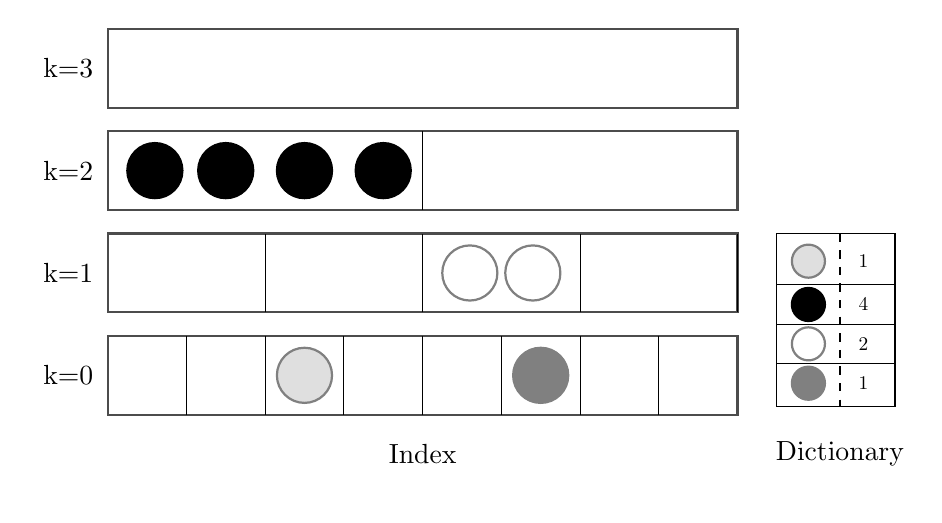
\begin{tikzpicture}
[
grayball/.style={circle, draw=gray, fill=gray,  thick, minimum size=7mm},
lightgrayball/.style={circle, draw=gray, fill=gray!25,  thick, minimum size=7mm},
gwball/.style={circle, draw=gray, fill=white,  thick, minimum size=7mm},
blackball/.style={circle, draw=black, fill=black,  thick, minimum size=7mm},
whiteball/.style={circle, draw=white, fill=white, very thick, minimum size=7mm},
dummyball/.style={circle, draw=gray, fill=gray, very thick, minimum size=7mm},
bin/.style={rectangle, draw=black!70, fill=white, thick, minimum height=8cm, minimum width = 1cm, rotate=90},
textbox/.style={rectangle, draw=white, fill=white, thick, minimum height=1cm},
myarrow1/.style={single arrow, draw=blue, fill=green, 
      minimum width = 10pt, single arrow head extend=3pt,
      minimum height=10mm}
]
\node at (0,-1) [textbox]      (tb1)    {Index};
%level 0
\node at (-4.5,0) [whiteball] (w1) {k=0};
\node at (0,0) [bin] (bin1) {};
\draw[] (-3,-0.5) -- (-3,0.5) ;
\draw[] (-2,-0.5) -- (-2,0.5) ;
\draw[] (-1,-0.5) -- (-1,0.5) ;
\node at (-1.5, 0) [lightgrayball] (lgb) {};
\draw[] (0,-0.5) -- (0,0.5) ;
\draw[] (1,-0.5) -- (1,0.5) ;
\draw[] (2,-0.5) -- (2,0.5) ;
\node at (1.5, 0) [grayball] (gb) {};
\draw[] (3,-0.5) -- (3,0.5) ;

 %level 1
 \node at (-4.5,1.3) [whiteball] (w1) {k=1};
\node at (0, 1.3) [bin] (bin2) {};
\draw[] (-2,0.8) -- (-2,1.8) ;
\draw[] (0,0.8) -- (0,1.8) ;
\draw[] (2,0.8) -- (2,1.8) ;
\node at (0.6,1.3) [gwball] (wb1) {};
\node at (1.4,1.3) [gwball] (wb2) {};
\draw[] (4,0.8) -- (4,1.8) ;

%level 2
\node at (-4.5,2.6) [whiteball] (w1) {k=2};
\node at (0, 2.6) [bin] (bin3) {};
\draw[] (0,2.1) -- (0,3.1) ;
\node at (-3.4,2.6) [blackball] (bb1) {};
\node at (-2.5,2.6) [blackball] (bb1) {};
\node at (-1.5,2.6) [blackball] (bb1) {};
\node at (-0.5,2.6) [blackball] (bb1) {};
%level 3
\node at (-4.5,3.9) [whiteball] (w1) {k=3};
\node at (0, 3.9) [bin] (bin4) {};

 %%dictionary

 \draw[] (4.5,1.8) rectangle (6,-0.4) {};
 \node at (5.3,-1) [textbox]      (d1)       {Dictionary};
 \node[scale=0.6] at (4.9,0.9) [blackball]   (d1)  {};
 \node[scale=0.7] at (5.6,0.9) [whiteball]   (d1)  {4};
 
  \node[scale=0.6] at (4.9,0.4) [gwball]   (d1)  {};
  \node[scale=0.7] at (5.6,0.4) [whiteball]   (d1)  {2};
  
   \node[scale=0.6] at (4.9,-0.1) [grayball]   (d1)  {};
   \node[scale=0.7] at (5.6,-0.1) [whiteball]   (d1)  {1};
   \node[scale=0.6] at (4.9,1.45) [lightgrayball]   (d1)  {};
   \node[scale=0.7] at (5.6,1.45) [whiteball]   (d1)  {1};
   \draw[] (4.5,0.65) -- (6,0.65) ;
   \draw[] (4.5,0.15) -- (6,0.15) ;
   \draw[] (4.5,1.15) -- (6,1.15);
   \draw[thick,dashed] (5.3,1.8) -- (5.3,-0.4) {};

\end{tikzpicture}
}
}


\vspace{0.7cm}
\subfloat[2C (Part I). Braces indicate superbin.]
{
\scalebox{0.8}
{
\begin{tikzpicture}
[
grayball/.style={circle, draw=gray, fill=gray,  thick, minimum size=7mm},
lightgrayball/.style={circle, draw=gray, fill=gray!25,  thick, minimum size=7mm},
gwball/.style={circle, draw=gray, fill=white,  thick, minimum size=7mm},
blackball/.style={circle, draw=black, fill=black,  thick, minimum size=7mm},
whiteball/.style={circle, draw=white, fill=white, very thick, minimum size=7mm},
dummyball/.style={circle, draw=gray, fill=gray, very thick, minimum size=7mm},
bin/.style={cylinder, draw=black!70, fill=white, thick, minimum height=3cm, minimum width = 1cm, rotate=90},
textbox/.style={rectangle, draw=white, fill=white, thick, minimum height=1cm},
myarrow1/.style={single arrow, draw=blue, fill=green, 
      minimum width = 10pt, single arrow head extend=3pt,
      minimum height=10mm}
]
\node at (3,-1.2) [textbox]      (tb1)    {Index};
\draw [decorate, decoration = {brace, amplitude = 10pt}, dashed, thick] (0.5,2.8) --  (5.4,2.8);
\draw [decorate, decoration = {brace, amplitude = 7pt}] (0.5,2.3) --  (2.7,2.3);
 \node at (1,0.5) [bin] (bin1) {};
\node at (1,-0.4) [blackball]      (ball1)    {};
\node at (1,0.5) [gwball]      (d1)     {};
\node at (2.3,1.5) [gwball]      (d1)     {};

 \node at (2.3,0.5) [bin] (bin2) {};
 \node at (2.3,-0.4) [blackball]      (d2)    {};
 \node at (2.3,0.5) [gwball]      (d1)     {};
 
\draw [decorate, decoration = {brace, amplitude = 7pt}] (3.2,2.3) --  (5.4,2.3);
 \node at (3.6,0.5) [bin] (bin3) {};
 \node at (3.6,-0.4) [blackball]      (d2)    {};
% \node at (3.6,0.5) [gwball]      (ball2)      {};
 
 \node at (4.9, 0.5) [bin] (bin4) {};
 \node at (4.9,-0.4) [blackball]      (d2)    {};
 %\node at (4.9,0.5) [gwball]      (ball2)    {};

 %%dictionary
 \draw[] (6,1.8) rectangle (7.5,-0.4) {};
 \node at (6.8,-1) [textbox]      (d1)       {Dictionary};
 \node[scale=0.6] at (6.4,0.9) [blackball]   (d1)  {};
 \node[scale=0.7] at (7.1,0.9) [whiteball]   (d1)  {4};
 
  \node[scale=0.6] at (6.4,0.4) [gwball]   (d1)  {};
  \node[scale=0.7] at (7.1,0.4) [whiteball]   (d1)  {2};
  
   %\node[scale=0.6] at (6.4,-0.1) [grayball]   (d1)  {};
   %\node[scale=0.7] at (7.1,-0.1) [whiteball]   (d1)  {1};
  % \node[scale=0.6] at (6.4,1.45) [lightgrayball]   (d1)  {};
   %\node[scale=0.7] at (7.1,1.45) [whiteball]   (d1)  {1};
   \draw[] (6,0.65) -- (7.5,0.65) ;
    \draw[] (6,0.15) -- (7.5,0.15) ;
    \draw[] (6,1.15) -- (7.5,1.15);
    \draw[thick,dashed] (6.8,1.8) -- (6.8,-0.4) {};

 \end{tikzpicture}
}
}
\hspace*{90pt}
\subfloat[2C (Part II)]
{
\scalebox{0.8}{
\begin{tikzpicture}
[
grayball/.style={circle, draw=gray, fill=gray,  thick, minimum size=7mm},
lightgrayball/.style={circle, draw=gray, fill=gray!25,  thick, minimum size=7mm},
gwball/.style={circle, draw=gray, fill=white,  thick, minimum size=7mm},
blackball/.style={circle, draw=black, fill=black,  thick, minimum size=7mm},
whiteball/.style={circle, draw=white, fill=white, very thick, minimum size=7mm},
dummyball/.style={circle, draw=gray, fill=gray, very thick, minimum size=7mm},
bin/.style={cylinder, draw=black!70, fill=white, thick, minimum height=3cm, minimum width = 1cm, rotate=90},
textbox/.style={rectangle, draw=white, fill=white, thick, minimum height=1cm},
myarrow1/.style={single arrow, draw=blue, fill=green, 
      minimum width = 10pt, single arrow head extend=3pt,
      minimum height=10mm}
]
\node at (3,-1.2) [textbox]      (tb1)    {Index};
\node at (1,0.5) [bin] (bin1) {};
\draw [decorate, decoration = {brace, amplitude = 7pt}, very thick] (0.5,2.7) --  (1.5,2.7);
\draw [decorate, decoration = {brace, amplitude = 7pt}] (0.5,2.3) --  (1.5,2.3);
\node at (1,-0.4) [blackball]      (ball1)    {};
\node at (1,0.5) [gwball]      (d1)     {};


 \node at (2.3,0.5) [bin] (bin2) {};
 \node at (2.3,-0.4) [blackball]      (d2)    {};
 \node at (2.3,0.5) [gwball]      (d1)     {};

 \draw [decorate, decoration = {brace, amplitude = 7pt}, very thick] (3.1,2.7) --  (4.1,2.7);
 \node at (3.6,0.5) [bin] (bin3) {};
 \node at (3.6,-0.4) [blackball]      (d2)    {};
 \node at (3.6,0.5) [lightgrayball]      (ball2)      {};

 \draw [decorate, decoration = {brace, amplitude = 7pt}] (4.4,2.3) --  (5.4,2.3);
 \node at (4.9, 0.5) [bin] (bin4) {};
 \node at (4.9,-0.4) [blackball]      (d2)    {};
 \node at (4.9,0.5) [grayball]      (d1)     {};
 %\node at (4.9,1) [gwball]      (ball2)    {};

 %%dictionary
 
 \draw[] (6,1.8) rectangle (7.5,-0.4) {};
 \node at (6.8,-1) [textbox]      (d1)       {Dictionary};
 \node[scale=0.6] at (6.4,0.9) [blackball]   (d1)  {};
 \node[scale=0.7] at (7.1,0.9) [whiteball]   (d1)  {4};
 
  \node[scale=0.6] at (6.4,0.4) [gwball]   (d1)  {};
  \node[scale=0.7] at (7.1,0.4) [whiteball]   (d1)  {2};
  
   \node[scale=0.6] at (6.4,-0.1) [grayball]   (d1)  {};
   \node[scale=0.7] at (7.1,-0.1) [whiteball]   (d1)  {1};
   \node[scale=0.6] at (6.4,1.45) [lightgrayball]   (d1)  {};
   \node[scale=0.7] at (7.1,1.45) [whiteball]   (d1)  {1};
   \draw[] (6,0.65) -- (7.5,0.65) ;
    \draw[] (6,0.15) -- (7.5,0.15) ;
    \draw[] (6,1.15) -- (7.5,1.15);
    \draw[thick,dashed] (6.8,1.8) -- (6.8,-0.4) {};

\end{tikzpicture}
}
}
\caption{Each keyword is visualized with a color and an entry in the index of that keyword is visualized as ball of that particular color. In \OneChoice\ and \TwoChoice\, after assigning the entries to the bins, the bins are filled with dummy entries and each bin is randomly shuffled. The length of the input dataset is $N$. For \TwoChoice\ and \NlogN\ schemes each keyword list is padded to be power 2. A dictionary is maintained in each of these schemes. \textbf{(a)} In \OneChoice\ scheme $m=N/\log N \log \log N$ bins are allocated, each of size $3\log N \log \log N$. Same colored balls are stored in adjacent bins. The first bin is calculated with a hash function $h(\bullet)$. The $k$th ball is stored at bin $(h(\bullet)+k)\%m$. For example, for the black ball $h(\bullet)$ returns 1. Hence, the first ball (k=0) is stored in bin $(h(\bullet)+0)\%3)=1$, the second ball (k=1) in bin $(h(\bullet)+1)\%3)=2$, and the third ball (k=2) is stored (wraps-around) in bin$(h(\bullet)+2)\%3)=0$. \textbf{(b)} The \NlogN\ scheme instantiates $(\log N +1)$ levels each of size $N$. The $k$th level stores lists of size $2^k$, in a contiguous memory chunk; i.e. each level is divided into $N/2^k$ chunks. We have 8 elements, hence we have $(\log 8 +1)=4$ levels. Because the list of black balls is of size 4, it is stored in level 2 (as $2^2 = 4$). Similarly, the list of white balls is stored in level 1. The gray and the light gray lists consist of single element each, and hence they get stored in level 0. A hash function is used to decide which memory chunk stores the data. 
\textbf{(c)} \TwoChoice\ allocates  $m={N}/{(\log\log N)^A (\log \log \log N)^2}$ bins, of size $z{\cdot}(\log\log N)^A$ ($\log$$\log$$\log N)^2$, ($2\leq z \leq 4$ , we use $A=1$).
Keyword lists are stored in \emph{decreasing order} of their lengths; e.g. the list of black balls will be stored first, and then the list of white balls and so on. For each keyword $w$, first
it divides the bins into groups of $sb = \frac{m}{n_w}$ \emph{superbins}; e.g. for the list of black balls we have $4/4 =1$ superbin consisting of 4 bins (marked with a dashed curly brace), while for the list of white balls, we have $4/2 =2$ superbins, consisting of 2 bins each (marked with two separate curly braces). Then two prospective superbins for a particular keyword are computed using two hash values $h_1(\bullet)\% sb$ and $h_2(\bullet)\%sb$; and superbin with minimal load is chosen. Both the superbins for the white balls have same load, so anyone can be chosen. \textbf{(d)} The two superbins for the gray ball is computed to be bin $0$ and bin $2$. Bin $2$ has one black ball, while bin $0$ has one black and a white ball, hence the superbin with minimal load is bin $2$. Similarly, for the light gray ball, whose superbins are bin $0$ and bin $3$, is stored in bin $3$. The 
corresponding hash functions and the dictionary is used during a search operation.}
\label{fig:allSEschemes}
\end{figure*}



%\section{DSE Security}\label{app:sse}
\mdfdefinestyle{mystyle2}{userdefinedwidth=20cm,rightmargin=0.7cm}
\begin{figure*}[!h]
\begin{mdframed}[style=mystyle2]
$EDB$ consists of two parts; 
$EDB.\Ind$ stores the encrypted \OneChoice~ array and
$EDB.\Dict$ stores an encrypted dictionary \\
Let $\RND = (\Enc, \Dec, \keyGen)$ is CPA-secure encryption scheme \\
\vspace{-1cm}
\begin{multicols}{2}
 \underline{$(K,\sigma;EDB) \leftarrow \texttt{Setup}(1^\lambda,DB)$}
 \begin{algorithmic}[1]
  \State $F:\{0,1\}^{*}\times \{0,1\}^{\lambda} \xrightarrow[]{} \{0,1\}^{*}$ is a PRF
  \State $(k_{rnd},k_{prf}) \gets {\texttt{KeyGen}}(1^\lambda)$ 
   \State $N \gets |DB|$
  \State $binSize \gets max(3\cdot \log N \log \log N,1)$ 
  \State $maxBins \gets max(\ceil{\frac{N}{\log N \log \log N}},1)$ 
  \State Initialize empty map \textbf{M} of size $N$
%  \State Fill up array $\BUF$ of size $3{\cdot} N $ with $\RND.\Enc(k_{rnd},(\dummy, \dummy,\dummy))$
%  \Statex{\tpurp{$\rhd$ The third attribute is the extra piece }}
 % \Statex{\tpurp{of data that is needed per entry in our DSE constructions}}
  %\State Initialize an empty Map $L$ that maps each unique keyword of $DB$ to the list of entries for that keyword in $DB$ 
  %\State For each unique keyword $w$ add all entries $(w,id,op)\in DB$ to $L$
  %  by calling $L[w].\Append((w,id,op))$
   \State Create separate lists with entries of each unique keyword $L=\{l_{w_1},l_{w_2}, \ldots, l_{w_n}\}$
\For{$i=1 \ldots n$}
\State $cnt \gets 0$
  \For{each entry $(w_i,id.op) \in l_{w_i}$}
  \State  $((bin,pos),\sigma) \gets \texttt{Map}(k_{prf},w_i,cnt,|l_{w_i}|,N,\sigma)$
 \State Place $\RND.\Enc(k_{rnd},(w_i,id,op))$ in the next available spot in $bin$ in $\BUF$
 \State $cnt \gets cnt+1$
   %\State Parse $l$ as $(w,l')$, and $l'$ as $\{e_1,e_2,\ldots, e_n \}$
   %\State $start \gets ((h(w)+cnt_w)\%m)\cdot binSize $
% \State $((bin,0),\sigma) \gets \texttt{Map}(k_{prf},w,1,|DB(w)|,N,\sigma)$
 \EndFor
    \State  \textbf{M}$[H(F(k_{prf},w_i),1)] \gets \RND.\textsf{Enc}(k_{rnd},|l_{w_i}|)$
   \EndFor
   \State Pad every bin to maximum capacity with $\RND.\Enc(k_{rnd},(\dummy, \dummy,\dummy))$ and randomly shuffle each bin
   \State $EDB.\Ind \gets \BUF$ and $EDB.\Dict \gets $ \textbf{M}
   \State Store $K$ as $(k_{rnd},k_{prf})$ and $maxBins$ and $binSize$ in $\sigma$ 
   \State \Return $EDB$ to server
   \Statex
   \Statex
    \end{algorithmic}
    

\underline{$(k_{rnd},k_{prf}) \leftarrow \texttt{KeyGen}(1^\lambda)$}
\begin{algorithmic}[1]
 \State $k_{prf} \gets $Choose a random PRF key for $F$
 \State Set $k_{rnd} \leftarrow$ \RND.\keyGen$(1^\lambda)$ 
  %\State $k_{prf_{cnt}} \gets $Choose a random PRF key for $F$
 %\State Randomly choose hash function $h$ from family $\mathcal{H}$
 \State \Return $(k_{rnd},k_{prf})$
\end{algorithmic}

% \underline{$bin \leftarrow \texttt{Map}(w,cnt_w,m,h)$}
 \underline{$((binNum,pos),\sigma) \leftarrow \texttt{Map}(k_{prf}, w, rank,n_w,\sigma)$}
\begin{algorithmic}[1]
%\State $maxBins \gets \ceil{\frac{N}{\log N \log \log N}}$
\If {$w \neq \dummy $}
 \State{ $binNum \gets (H(F(k_{prf},w),0)+rank)\%maxBins $}
 \Else 
 \State{ $binNum \gets \bot$}
 \EndIf
 \State {\Return $((binNum,0),\sigma)$}
\end{algorithmic}

%  \underline{$binNum \leftarrow \texttt{Map}(k_{prf}, w, cnt_w, maxBins)$}
%\begin{algorithmic}[1]
%\If {$w \neq \dummy $}
%\State{ $binNum \gets (H(F(k_{prf},w),0)+cnt_w)\%maxBins $}
 %\EndIf
 %\ElsI { $binNum \gets (maxBins)+1$}
 %\EndIIf
% \State {\Return $(binNum,0)$}
%\end{algorithmic}

\underline{$res \leftrightarrow \texttt{Search}(k,w,\sigma;EDB)$}
  \begin{algorithmic}[1]
  \item[Client $\leftrightarrow$ Server:]
  \State parse $k$ as $(k_{rnd},k_{prf})$
 % \State $bins \gets \ceil{\frac{N}{\log N \log \log N}}$;\quad $binSize \gets 3{\cdot}\log N \log \log N$
  \State $ n_w \gets \RND.\Dec(k_{rnd}, EDB.\Dict[H(F(k_{prf},w),1)])$
  %	\item[Client:]
  \State Client runs $((st,pos),\sigma) \gets\texttt{Map}(k_{prf},w,0,n_w,\sigma){\cdot} binSize$
%  \State Client runs $end \gets (start+cnt_w)\cdot binSize -1$
 % \item[Client $\leftrightarrow$ Server:]
  \State Client gets $eres \leftarrow$ $EDB.\Ind$[$st,\ldots,((st+n_w){\cdot} binSize)$]
%   \item[Client:]
   \State Client Initializes empty set $res$ to store results
   \For {each $e \in eres$}
    \State $(w',id, op) \gets \RND.\Dec(k_{rnd},e)$
    \IIf{$w' = w$}
    {$res \gets res \cup \{(w,id,op)\}$}
   \EndFor
 \State \Return $res$
  %\EndFor
\end{algorithmic}
\end{multicols}
\vspace{-0.5cm}
\underline {{${\sf NEW}_i$ $ \leftrightarrow$ {\OneChoice.\omerge$(K, \sigma, {\sf OLDEST}_{i - 1},{\sf OLDER}_{i - 1})$}}}
\begin{algorithmic}[1]
\item[Client $\leftrightarrow$ Server:]
\Statex \textcolor{blue}{//** \ \ Phase 1---Preparing sorted input array\ \   **//}	
\State Parse $K$ as $(k_{rnd},P)$;\quad $oldw \gets \bot$ ;\quad  $cnt \gets \bot$ \label{sdd1c:counter} %\Comment{all encryptions and decryptions are done with key $k_{rnd}$, $P$ is an array of PRF keys}
%\State Client initializes a tuple called $\pr$ as $(\bot, 0)$ and stores it in local state $\sigma$
\State Initialize arrays \BUF$_1$ of size $2{\cdot}3{\cdot}2^1$, and \BUF$_2$ of size $3{\cdot}2^i$ to be empty
\State Copy $\OLDEST_{i-1}.\Ind \cup \OLDER_{i-1}.\Ind$ to $\BUF_1$; obliviously sort $\BUF_1$ w.r.t. 
 lexicographic order of keywords
%\State Perform two linear scans (one in reverse and one in correct order) on $\BUF_1$, to add the $rank$ values to each entry of keyword $w$. The entries now look like $((w,id,op),rank)$, where $0 \leq rank < |DB(w)|$. 
%\State Perform two linear scans (one in reverse and one in correct order) on $\BUF_1$, to add the $rank$ and $n_w$ values to each entry of keyword $w$. The entries now look like $((w,id,op),rank,n_w)$, where $0 \leq rank < n_w$. 
%\State {Linear scan $\BUF_1$ and pad appropriately to make each list's size nearest power of 2, without leaking the actual list length}
   % \State {$cnt \gets 0$}
   %\State {Perform oblivious sort on $\BUF_1$ based on lexicographic order of the keywords and  descending order of the $n_w$ values. Keep first $\Sigma.N$ elements.}
   % 
  \Statex \textcolor{blue}{//** \ \ Phase 2---Move elements and Prepare keyword counters \ \ **//}	
    \For{each $j = 1 \ldots |\BUF_1|$} %\tpurp{optimize with pair}
%    \State $((w,id,op),rank,n_w) \gets \RND.\Dec(k_{rnd},\BUF_1[j])$ %and parse $\pr$ as $(w',cnt)$
     \State $(w,id,op) \gets \RND.\Dec(k_{rnd},\BUF_1[j])$; \quad {$p \gets^{\$} \{0,1\}^\lambda$}
      \If{~~$(w$ is observed for first time $\wedge$ $oldw \neq \bot)$}    \State {$\BUF_{2}.\Append(\RND.\Enc(k_{rnd},(oldw,cnt,p)))$;\quad $oldw \gets w$ ; \quad $cnt \gets 0$} 
      \label{sdd1c:resetCounter}
      \EndIf
      \ElsI{~~$\BUF_{2}.\Append(\RND.\Enc(k_{rnd},(\bot,\bot,\bot)))$; \quad $cnt\plus\plus$}
      %\EndIf
    %\If{$w' \neq w$ and $w' \neq \bot$} \Comment{i.e. Client is seeing $w$ for the first time}
    %\IIf{$rank = 0$}{~$\BUF_{2}.\Append(\RND.\Enc(k_{rnd},((w,n_w),p)))$}%; \quad {$cnt \gets 1$}
    %\ElsI{$\BUF_{2}.\Append(\RND.\Enc(k_{rnd},((\bot,0),0)))$}%; \quad {$cnt \textsc{++}$}
    %\EndIf
    %\State Client stores $(w,cnt)$ as $\pr$ in local state $\sigma$
   % \State $\pr \gets (w,cnt)$ \Comment{$\pr$ is updated with latest keyword and counter}
    \State $((bin,pos),\sigma)\gets\OneChoice.\texttt{Map}(P[i][3],w,cnt,\bot,\sigma)$ \label{sdd1c:map}%\Comment{$m_i$ = number of bins for \OneChoice~ for $2^i$ elements}
  \State \BUF$_{1}.\Append(\RND.\Enc(k_{rnd},(w,id,op,bin,pos)))$ \Comment{bin tag is added per entry}
    \EndFor
%    \State Parse $\pr$ as $(w',cnt')$ \Comment{for the last keyword in \textsf{SORTED}}
 %   \If{$w' \neq \bot$} 
 %   \State {$ p \gets^{\$} \{0,1\}^\lambda$ 
  %  \State $\BUF_{2}.\Append(\RND.\Enc(k_{rnd},((w',cnt'),p))$}
% \Else
%    \State {$\BUF_{2}.\Append(\RND.\Enc(k_{rnd},((\bot,0),0))$}
 %   \EndIf
    \Statex \textcolor{blue}{//** \ \ Phase 3---Add dummies\ \ **//}	\Comment{this phase adds binsize dummy entries per bin}
    \For{$bin= 0 \ldots \ceil{\frac{2^i}{\log 2^i \log \log 2^i}}-1$}
    \State Append $\RND.\Enc(k_{rnd},(\bot,\bot,\bot,bin,0))$ to $\BUF_1$  $3{\cdot} \log 2^i\log \log 2^i$ times \Comment{size of bins in \OneChoice~ when $N=2^i$}
    \EndFor
     \Statex \textcolor{blue}{//** \ \ Phase 4---Final placement \ \ **//}	
    \State Perform oblivious sort on $\BUF_1$ w.r.t. the $bin$ values of $(bin,0)$ pair in ascending order%; discard the bin tags
    \State Linearly scan $\BUF_1$, and tag \textbf{first} $3{\cdot} \log 2^i\log \log 2^i$ entries for each $bin\in \{0, \ldots, \ceil{\frac{2^i}{\log 2^i \log 2^i \log 2^i}}\}$ with 1, and with 0 the rest of them (existing $(bin,0)$ tags are replaced with 0/1 tags, entries now look like $(w,id,op,x)$, where $x \in \{0,1\}$)
        \State {Perform order preserving oblivious compaction on $\BUF_1$; keep first $\Sigma.N$ entries; discard the 0/1 tags }
    \State Perform oblivious sort on $\BUF_2$ w.r.t. the random keys in ascending order; keep first $2^i$ entries; discard random keys
    \State 	\NEW$_i.\OneChoice$ $\gets$ \BUF$_1$ and randomly shuffle each bin
   \For{each $s \in \BUF_2$}
\State $(w, cnt_w) \gets \RND.\Dec(k_{rnd}, s)$
\State $(key,value) \gets \PiBas.\MAP((P[i][3],k_{rnd}),w,cnt_w,1)$ \Comment{parameter 1 is used by the PRF $F$}
%\State $key \gets H(F(P[i][3],w),1)$ and $value \gets \RND.\Enc(R[i][3],cnt_w)$
\State 	\NEW$_i.$\Dict[$key$] $\gets value$
\EndFor
\State \Return \NEW$_i$
%\Statex (keep $3.2^i$ size of dictionary and explain we can optimize to $2^i$ size with extra 5-6 lines, write a paragraph about it, but if you can do it in the pseudocode do it)
%\Statex \tpurp{Client storage is logN because there are logN indexes}
\end{algorithmic}

\end{mdframed}
%\vspace{-.3cm}
\caption{One-Choice Allocation (\OneChoice.\omerge\ is the optimized version)}
\label{alg:1C} \label{alg:sdd1C}
\end{figure*}






\begin{figure*}[!h]
\begin{mdframed}
$EDB$ consists of two parts; 
$EDB.\Ind$ stores the encrypted \TwoChoice~ array and
$EDB.\Dict$ stores an encrypted dictionary that maps each unique keyword
to its keyword-counter.\\
Let $\RND = (\Enc, \Dec, \keyGen)$ is CPA-secure encryption scheme \\
%Let $m_i'$ denotes a value bigger than total number of bins \\
\vspace{-0.8cm}
 \begin{multicols}{2}
\underline{$(K,\sigma;EDB) \leftarrow \texttt{Setup}(1^\lambda,DB)$}
 \begin{algorithmic}[1]
  \State $F_1:\{0,1\}^{*}\times \{0,1\}^{\lambda} \xrightarrow[]{} \{0,1\}^{*}$ is a PRF
 \State $F_2:\{0,1\}^{*}\times \{0,1\}^{\lambda} \xrightarrow[]{} \{0,1\}^{*}$ is a PRF
  \State $(k_{rnd},k_{prf}) \gets {\texttt{KeyGen}}(1^\lambda)$ 
  \State $N \gets |DB|$
  \State $binSize \gets$ max$(z\cdot \log \log N {\cdot}(\log \log \log N)^2,1)$ 
  \State $maxBins \gets$ max$(\ceil{\frac{N}{\log \log N (\log \log \log N)^2}},1)$ \Comment{$2 \leq z \leq 4$}
  \State Initialize empty map \textbf{M} of size $N$
  \State $z \gets$ choose a value between 2 and 4
  \State Initialize array $\BUF$ of size $z\cdot N $
%  \Statex{\tpurp{$\rhd$ The last three attributes are the extra information needed per entry in \LSDd[\TwoChoice]}}
  \State Create separate lists with entries of each unique keyword $L=\{l_{w_1},l_{w_2}, \ldots, l_{w_n}\}$, such that $|l_{w_1}|>|l_{w_2}|>\ldots |l_{w_n}|$
  \State Pad list of each keyword $w_i$ to nearest power of 2 with fake entries, (e.g. with $(w_i,\dummy,\dummy)$ for $w_i$)
  \For{$i=1\ldots n$}
%  \State $(sbin_1,sbin_2) \gets \texttt{Map}(k_{prf},w_i,|l_{w_i}|,bins)$
%  \State {$sbin\gets$ choose the $superbin$ with minimal load among $sbin_1$ and $sbin_2$}
  \State $cnt \gets 0$
  \For{entry $(w_i,id.op) \in l_{w_i}$}
  \State  $((bin,pos),\sigma) \gets \texttt{Map}(k_{prf},w_i,cnt,|l_{w_i}|,N,\sigma)$
 \State Place $\RND.\Enc(k_{rnd},(w,id,op))$ in the next available spot in $bin$ in $\BUF$
 \State $cnt \gets cnt+1$
 \EndFor
    \State  \textbf{M}$[H(F_1(k_{prf},w_i),1)] \gets \RND.\textsf{Enc}(k_{rnd},|l_{w_i}|)$
   \EndFor
\State Pad every bin with dummy entries to its maximum capacity, and randomly shuffle the entries 
   \State $EDB.\Ind \gets \BUF$ and $EDB.\Dict \gets $ \textbf{M}
   \State Store $K$ as $(k_{prf}, k_{rnd})$ and $maxBins$ and $binSize$ in $\sigma$ 
   \State \Return $EDB$ to server
   \Statex
    \end{algorithmic}

%\begin{multicols}{2}
\underline{$(k_{rnd},k_{prf}) \leftarrow \texttt{KeyGen}(1^\lambda)$}
\begin{algorithmic}[1]
% \State $(k_{prf_1},k_{prf_2}) \gets $Choose two random PRF keys for $F_1$ and $F_2$
 \State $(k_{prf}) \gets $Choose a PRF keys for $F_1$ and $F_2$
 \State Set $k_{rnd} \leftarrow$ \RND.\keyGen$(1^\lambda)$ 
  %\State $k_{prf_{cnt}} \gets $Choose a random PRF key for $F$
 %\State Randomly choose hash function $h$ from family $\mathcal{H}$
 \State \Return $(k_{rnd},k_{prf})$ %\Comment{$k_{prf} = (k_{prf_1},k_{prf_2})$}
\end{algorithmic}

\underline{$((binNum,pos),\sigma) \leftarrow \texttt{Map}(k_{prf}, w, rank, n_w,\sigma)$}
\begin{algorithmic}[1]
%\State $maxBins \gets \ceil{\frac{N}{\log \log N (\log \log \log N)^2}}$;\quad 
\State $n_w \gets 2^{\ceil{\log n_w}}$
\State $superBins \gets \frac{maxBins}{n_w}$
\If {$w \neq \dummy $}
 \State{ $sbin_1\gets (H(F_1(k_{prf},w),0))\%superBins $}
 \State{ $sbin_2\gets (H(F_2(k_{prf},w),0))\%superBins $}
 \If{$rank <0$} \Comment{for search query}
 \State \Return $((sbin_1,sbin_2),\sigma)$
 \EndIf
 \State $sbin$=$\sigma.\BIN[sbin_1]$<$\sigma.\BIN[sbin_2] \textsf{?} sbin_1 : sbin_2$
 \State $binNum \gets sbin*n_w+rank$
\State $\sigma.\BIN[sbin]\plus\plus$ 
 \EndIf
 \ElsI{ $binNum \gets \bot$}
 %\EndIf
 \State {\Return $((binNum,0),\sigma)$}
% \State{}
\end{algorithmic}


 \underline{$res \leftrightarrow \texttt{Search}(k,w,\sigma;EDB)$}
  \begin{algorithmic}[1]
  \item[Client $\leftrightarrow$ Server:]
 % \State $bins \gets \ceil{\frac{N}{\log \log N (\log \log \log N)^2}}$
%  \State $binSize \gets Z{\cdot}\log \log N \log \log \log N$
  \State parse $k$ as $( k_{rnd},k_{prf})$
  \State $ n_w \gets \RND.\Dec(k_{rnd}, EDB.\Dict[H(F_1(k_{prf},w),1)])$
  %	\item[Client:]
  \State $((sbin_1,sbin_2),\sigma) \gets\texttt{Map}(k_{prf},w,-1,n_w,\sigma)\cdot binSize$
  %\State{ $sbin_1\gets (H(F_1(k_{prf},w),0))\%bins $}
 %\State{ $sbin_2\gets (H(F_2(k_{prf},w),0))\%bins $}
%  \State Client runs $end \gets (start+cnt_w)\cdot binSize -1$
 % \item[Client $\leftrightarrow$ Server:]
  \State Client fetches entries of $superbin$s $sbin_1$ and $sbin_2$ from $EDB.\Ind$ in array $eres$
   \item[Client:]
   \State Client Initializes empty set $res$ to store results
   \For {each $e \in eres$}
    \State $(w',id, op) \gets \RND.\Dec(k_{rnd},e)$
    \IIf{$w' = w$}
    {$res \gets res \cup \{(w,id,op)\}$}
   \EndFor
 \State \Return $res$
  %\EndFor
\end{algorithmic}
\end{multicols}
\end{mdframed}
%\vspace{-.5cm}
\caption{Two-Choice Allocation}
\label{alg:2C}
\end{figure*}




\begin{figure*}[]
\begin{mdframed}
$EDB$ consists of two parts; 
%$EDB.{A_0}, EDB.{A_1}, EDB.{A_2}, \ldots,$ 
$EDB.\Ind$ stores the encrypted $(\log N +1)$ arrays and
$EDB.\Dict$ stores an encrypted dictionary that maps each unique keyword
to its keyword-counter.\\
Let $\RND = (\Enc, \Dec, \keyGen)$ is CPA-secure encryption scheme \\
%Let $m_i'$ denotes a value bigger than total number of bins \\
\vspace{-0.8cm}

\begin{multicols}{2}
\underline{$(K,\sigma;EDB) \leftarrow \texttt{Setup}(1^\lambda,DB)$}
 \begin{algorithmic}[1]
 \State $F:\{0,1\}^{*}\times \{0,1\}^{\lambda} \xrightarrow[]{} \{0,1\}^{*}$ is a PRF
  \State $(k_{rnd},k_{prf}) \gets {\texttt{KeyGen}}(1^\lambda)$ 
  %\State $binSize \gets max(3\cdot \log \log N \log \log \log N,1)$ and $bins \gets max(\ceil{\frac{N}{\log \log N \log \log \log N}},1)$ 
   \State $N \gets |DB|$
    \State $levels \gets \ceil{\log N}+1$
  \State Initialize empty map \textbf{M} of size $N$
  \State Initialize array $\BUF$ of size $N {\cdot}(\ceil{\log N}+1)$
%  \Statex{\tpurp{$\rhd$ The last three attributes are the extra information needed per entry in \LSDd[\TwoChoice]}}
  \State Create separate lists with entries of each unique keyword $L=\{l_{w_1},l_{w_2}, \ldots, l_{w_n}\}$
  \State Pad list of each keyword $w_i$ to nearest power of 2 with fake entries, (e.g. with $(w_i,\dummy,\dummy)$ for $w_i$)
  \For{$i=1\ldots n$}
  \State $((level,pos),\sigma) \gets \texttt{Map}(k_{prf},w_i,0,|l_{w_i}|,N,\sigma)$
  %\State {$sbin\gets$ choose the $superbin$ with minimal load among $sbin_1$ and $sbin_2$}
  %\State $cnt \gets 0$
  \For{entry $(w_i,id.op) \in l_{w_i}$}
 \State Place $\RND.\Enc(k_{rnd},(w_i,id,op))$ in the next free position in range $\BUF[N{\cdot}level{\cdot}pos,~N{\cdot}level{\cdot}(pos\plus 1)\minus 1]$
 %\State $cnt \gets cnt+1$
 \EndFor
    \State  \textbf{M}$[H(F(k_{prf},w_i))] \gets \RND.\textsf{Enc}(k_{rnd},|l_{w_i}|)$
   \EndFor
\State Pad every empty position in each level with dummy entries  
   \State $EDB.\Ind \gets \BUF$ and $EDB.\Dict \gets $ \textbf{M}
   \State Store $K$ as $( k_{rnd},k_{prf})$ and $levels$  in $\sigma$ 
   \State \Return $EDB$ to server
    \end{algorithmic}


\underline{$(k_{rnd},k_{prf}) \leftarrow \texttt{KeyGen}(1^\lambda)$}
\begin{algorithmic}[1]
 \State $k_{prf} \gets $Choose a random PRF key for $F$
 \State Set $k_{rnd} \leftarrow$ \RND.\keyGen$(1^\lambda)$ 
  %\State $k_{prf_{cnt}} \gets $Choose a random PRF key for $F$
 %\State Randomly choose hash function $h$ from family $\mathcal{H}$
 \State \Return $(k_{rnd},k_{prf})$
\end{algorithmic}


 \underline{$((level,pos),\sigma) \leftarrow \texttt{Map}(k_{prf}, w, n_w,\sigma)$}
\begin{algorithmic}[1]
%\State $levels \gets \ceil{\log N} +1$; \quad 
\State $d \gets 2^{\ceil{\log n_w}}$
\If {$w \neq \dummy $}
\State $level \gets \log d$
\State{ $pos \gets (H(F(k_{prf},w),0))\%(2^{(levels -level)})$}
 \Else
 \State $level \gets \bot$
 \State {$pos \gets \bot$}
\EndIf
\State {\Return $((level,pos),\sigma)$}
\Statex {}
\end{algorithmic}

 \underline{$res \leftrightarrow \texttt{Search}(k,w,\sigma;EDB)$}
  \begin{algorithmic}[1]
  \item[Client $\leftrightarrow$ Server:]
  %\State $levels \gets \ceil{\log N}+1$
  \State parse $k$ as $( k_{rnd},k_{prf})$
  \State $ n_w \gets \RND.\Dec(k_{rnd}, EDB.\Dict[H(F(k_{prf},w))])$
  %	\item[Client:]
  \State Client runs $((level,pos),\sigma) \gets\texttt{Map}(k_{prf},w,0,n_w,\sigma)$
%  \State Client runs $end \gets (start+cnt_w)\cdot binSize -1$
 % \item[Client $\leftrightarrow$ Server:]
  \State Client fetches a set of $2^{level}$ entries from range
  \Statex {$[N{\cdot}level{\cdot}pos,~N{\cdot}level{\cdot}(pos\plus 1)\minus 1]$ from $EDB.\Ind$ and stores them in $eres$}
   \item[Client:]
   \State Client Initializes empty set $res$ to store results
   \For {each $e \in eres$}
    \State $(w',id, op) \gets \RND.\Dec(k_{rnd},e)$
    \IIf{$w' = w$}
    {$res \gets res \cup \{(w,id,op)\}$}
   \EndFor
 \State \Return $res$
  %\EndFor
\end{algorithmic}
\end{multicols}
\end{mdframed}
%\vspace{-.5cm}
\caption{\textsf{NlogN} scheme}
\label{alg:NlogN}
\end{figure*}

\if 0
%\mdfdefinestyle{mystyle2}{userdefinedwidth=9.5cm}
\begin{figure}[!bh]
\begin{mdframed}%[style=mystyle2]
\begin{algorithmic}[1]
%\small
  \State $max \gets 0$; \quad $len \gets |\BUF_1|$ 
    \For {$j= 1 \ldots len$}
    \State $((w,id,op),cnt,n_w) \gets \RND.\Dec(\BUF_1[j])$
    %\State $$\BUF_1$[j] \gets \RND.\Enc((w,id,op),cnt,max)$
     \If{Client sees $w$ for the first time}
    \State {\hskip-1em$cnt \gets n_w$;$\quad max \gets 2^{\ceil{\log n_w}}$}
    \EndIf
%    \IIf{$w=\bot$}{$~cnt\gets \bot$}
    \If{$w\neq \bot \wedge cnt < max$} %\Comment{\tblue{$\BUF_1$ is doubled}}
    \State {\hskip-1em $\BUF_1.\Append(\RND.\Enc(k,((w,\bot,\bot),cnt,n_w)))$}\label{pad:padentry}
    \Else
    \State {\hskip-1em$\BUF_1.\Append(\RND.\Enc(k,((\bot,\bot,\bot),\bot,\bot)))$}\label{pad:dummyentry}
    \EndIf
    \State $cnt\textsc{++}$
    \EndFor 
\end{algorithmic}
\end{mdframed}
%\vspace{-0.5cm}
\caption{Pad keyword lists ($\BUF_1$ length is doubled after padding)}
\label{alg:pad2}
\end{figure}




\begin{figure}[!hb]
\begin{mdframed}
\begin{algorithmic}[1]
%\small
    %%%\State $cnt \gets \bot$ %and initialize empty buffer $\BUF$
    \For {$j= |\BUF_1| \ldots 1$} \Comment{\tblue{scanned from the end}}
    \State $(w,id,op) \gets \RND.\Dec(k_{rnd},(\BUF_1[j]))$
    \IIf{Client sees $w$ for the first time}{$~cnt \gets 0$}
    \ElsI{$cnt\textsc{++}$}
    \IIf{$id=\bot$}{$~cnt\gets \bot$;$\quad w \gets \bot$}
    \State {$\BUF_1[j] \gets \RND.\Enc(k_{rnd},((w,id,op),cnt))$}
    \EndFor 
    \For {$j= 1 \ldots |\BUF_1|$} \Comment{\tblue{scanned from the start}}
    \State $((w,id,op),cnt) \gets \RND.\Dec(k_{rnd},\BUF_1[j])$
    \IIf{Client sees $w$ for the first time}{$~n_w \gets cnt$}
    \State {$\BUF_1[j] \gets \RND.\Enc(k_{rnd},((w,id,op),cnt,n_w))$}
    \EndFor 
\end{algorithmic}
\end{mdframed}
%\vspace{-0.5cm}
\caption{Adding $rank$ and $n_w$ values}
\label{alg:addrank}
\end{figure}

\fi





\begin{figure*}[!t]
\label{fig:Pibas}
	\begin{mdframed}
 Let {\sf RND = (KeyGen, Enc, Dec)} be a semantically-secure encryption scheme, $F$ be a PRF, and $H$ be a collision-resistant hash function. 
 %See Figure 4 of \cite{SDa} for \Setup and \Search.
 % \keyGen, \MAP, and \Search\ are exactly same as \cite{SDa}
 \vspace{-0.5cm}
 
 \begin{multicols}{2}
		\setlength{\itemindent}{-.3 in}
		%$(K, \sigma, EDB) \leftarrow $ Setup $(\lambda,DB)$.\\
		%$\mathcal{X} \leftarrow$ Search $(K,q,\sigma; EDB)$.\\
		%$DB \leftarrow$ DecryptALL $(K,\sigma,EDB)$.\\\\
		%\underline{$(st_{\sf C},\mathcal{I})\leftarrow${\sf Setup}$(k,\mathcal{D})$}
		\underline{$(K, EDB) \leftarrow \textsf{Setup}(1^\lambda, DB)$}
		\begin{algorithmic}[1]
			%			\State Set $EDB$ to be an empty vector of indexes $EDB_i$
			\State Initialize an empty map $T$
			\State Set $(k,k')\leftarrow$ \textsf{KeyGen}$(1^\lambda)$
   \State Create separate lists with entries of each unique keyword $L=\{l_{w_1},l_{w_2}, \ldots, l_{w_n}\}$
            \For{$i=1 \ldots n$}
			\For {each $(w_i,id,op)\in l_{w_i}$}
			\State Set counter $c\leftarrow 0$
			\State $(key,value) \leftarrow \textsf{Map}((k,k'),(w,id,op),c)$
			\State Store $(key,value)$ to $T; \quad c$++
			\EndFor
   \EndFor
			\State Set $K \leftarrow (k,k');\quad EDB \leftarrow T$
   \Statex{}
		\end{algorithmic}
	
  \underline{$(k,k') \leftarrow \textsf{KeyGen}(1^\lambda)$}
		\begin{algorithmic}[1]
			\State Choose random PRF key $k$ for $F$
			\State Set $k' \leftarrow$ RND.Enc$(1^\lambda)$\newline
   \Statex{}
		\end{algorithmic}
  	
		\underline{$(key,value) \leftarrow \textsf{Map}((k,k'),(w,id,op),c)$}
		\begin{algorithmic}[1]
			\State  $key \leftarrow H(F(k,w),c)$
			\State $value \leftarrow RND.Enc(k',(w,id,op))$\newline
		\end{algorithmic}	
\underline{$DB(w) \leftrightarrow \textsf{Search}(K,w,\sigma; EDB)$}
		\begin{algorithmic}[1]
			\item[Client:]
			\State Send $tk \leftarrow F(k,w)$ to server		
			\item[Server:]
			\State Set $\mathcal{X} \leftarrow \emptyset$;$\quad c \leftarrow 0$
			\While {$true$}
			\State Set $res \leftarrow T$.get$(H(tk), c)$
			\If {$res = \bot$} \textbf{break}
			\Else {} 
			$\mathcal{X} \leftarrow \mathcal{X} \cup res$; 	$\quad c$++		
			\EndIf
			\EndWhile
			\State Send $\mathcal{X}$ to client
			\item[Client:]
			\State $eres \gets $ Decrypt entries of $\mathcal{X}$ with $k'$ 	
                \State \Return $eres$
		\end{algorithmic}
	\end{multicols}	
 %\fi

\underline {${\sf NEW}_i$ $ \leftrightarrow$ {\PiBas.\omerge$(K,\sigma,{\sf OLDEST}_{i-1},{\sf OLDER}_{i-1})$}}
		\begin{algorithmic}[1]
		\item[Client $\leftrightarrow$ Server:]
	\State \textsc{OMAP$_{cnt_w}$} $\gets$ \OMAP.{\texttt{setup$(\lambda, 2^i)$}}
 \State Parse $K$ as $(k_{rnd},P)$ and let $k_{new}^{prf}$ be $P[i][3] $ %\Comment{In \cite{SDa} a key is denoted as $K[l][m]$}
	\For{each $e \in \OLDEST_{i-1}.\Ind \cup \OLDER_{i-1}.\Ind$} 
	\State Server sends $e$ to Client  
	\State Client decrypts $e$ with key $k_{rnd}$ and parses it as $(w,id,op)$
	 \State Client computes $num$ as the number of times $\NEW_i.\Ind$ has been fully  rebuilt using a counter that it stores locally
	\State Client runs $c_w\leftarrow$\textsc{OMAP$_{cnt_w}$}.\texttt{get}(($w,num$)) %\Comment{Client queries \textsc{OMAP}}
	\IIf { $c_{w}= \bot$ } client sets $c_{w} \leftarrow 0$
    %\EndIIf
%	\State $c_{w}\leftarrow c_{w}+1$ \Comment{Client sets the counter}
	\State Client runs \textsc{OMAP$_{cnt_w}$}.\texttt{put}$((w,num),\textsf{++}c_{w})$ %\Comment{Client queries \textsc{OMAP}}
	\State  Client runs $ekey \leftarrow H(F(k_{new}^{prf},w),c_{w})$ and $evalue \leftarrow$ RND$.\Enc(k_{new}^{rnd},(w,id,op))$
	\State Client sends to server $(ekey,evalue)$ who runs $\NEW_i.\texttt{put}(ekey,evalue)$
	%$(key,value) \leftarrow$                     %{\PiBas}.\texttt{Map}$(w,id,op,c_{w},K[i][3])$
%	\State 	$\NEW_i.\texttt{put}(ekey,evalue)$
	\EndFor
	\State \Return $\NEW_i$
	%\State \Return Out
	\end{algorithmic}
	\end{mdframed}
	%\vspace{-0.3cm}
 %\vspace{-.5cm}
	\caption{Static searchable encryption PiBas~\cite{cash2014dynamic}.}
	%\vspace{-.2cm}
	\label{fig:AllPibas}
\end{figure*}

\begin{figure*}
\begin{mdframed}
\underline {${\sf NEW}_i$ $ \leftrightarrow$ {\PiBas.\omerge$(K,\sigma,{\sf OLDEST}_{i-1},{\sf OLDER}_{i-1})$}}
		\begin{algorithmic}[1]
		\item[Client $\leftrightarrow$ Server:]
 \State Parse $K$ as $(k_{rnd},P)$ and let $k_{new}^{prf}$ be $P[i][3] $ %\Comment{In \cite{SDa} a key is denoted as $K[l][m]$}
 \State Server initializes $\BUF_1$ arrays of size $2^i$
 \State Perform oblivious sort on $\OLDEST_{i-1}.\Ind \cup \OLDER_{i-1}.\Ind$ in lexicographic order of keywords and store in $\BUF_1$
 \State Client linearly scans $\BUF_1$ to add \emph{rank} to each keyword entry; entries now look like $(w,id,op,rank)$
 \State Server randomly shuffles entries in $\BUF_1$
\For{each $e \in \BUF_1$} 
	\State Server sends $e$ to Client  
	\State Client decrypts $e$ with key $k_{rnd}$ and parses it as $(w,id,op, rank)$
	% \State Client computes $num$ as the number of times $\NEW_i.\Ind$ has been fully  rebuilt using a counter that it stores locally
	%\State Client runs $c_w\leftarrow$\textsc{OMAP$_{cnt_w}$}.\texttt{get}(($w,num$)) %\Comment{Client queries \textsc{OMAP}}
	%\IIf { $c_{w}= \bot$ } client sets $c_{w} \leftarrow 0$
    %\EndIIf
%	\State $c_{w}\leftarrow c_{w}+1$ \Comment{Client sets the counter}
	%\State Client runs \textsc{OMAP$_{cnt_w}$}.\texttt{put}$((w,num),\textsf{++}c_{w})$ %\Comment{Client queries \textsc{OMAP}}
	\State  Client runs $ekey \leftarrow H(F(k_{new}^{prf},w),rank)$ and $evalue \leftarrow$ RND$.\Enc(k_{rnd},(w,id,op))$
	\State Client sends to server $(ekey,evalue)$ who runs $\NEW_i.\texttt{put}(ekey,evalue)$
	%$(key,value) \leftarrow$                     %{\PiBas}.\texttt{Map}$(w,id,op,c_{w},K[i][3])$
%	\State 	$\NEW_i.\texttt{put}(ekey,evalue)$
	\EndFor
	\State \Return $\NEW_i$
	%\State \Return Out
	\end{algorithmic}
	\end{mdframed}
\caption{New \PiBas.\omerge without the OMAPs}
\label{alg:LSDd[PiBas]}
\end{figure*}





\begin{figure*}[!h]
\begin{mdframed}
\begin{multicols}{2}
\begin{algorithmic}[1]
%\small
    %%%\State $cnt \gets \bot$ %and initialize empty buffer $\BUF$
    \underline{Adding \emph{rank} and $a_w$ values}
    \For {$j= |\BUF_1| \ldots 1$} \Comment{\tblue{scanned from the end}}
    \State $(w,id,op) \gets \RND.\Dec(k_{rnd},(\BUF_1[j]))$
    \IIf{Client sees $w$ for the first time}{$~cnt \gets 0$}
    \ElsI{$cnt\textsc{++}$}
    \IIf{$id=\bot$}{$~cnt\gets \bot$;$\quad w \gets \bot$}
    \State {$\BUF_1[j] \gets \RND.\Enc(k_{rnd},((w,id,op),cnt))$}
    \EndFor 
    \For {$j= 1 \ldots |\BUF_1|$} \Comment{\tblue{scanned from the start}}
    \State $((w,id,op),cnt) \gets \RND.\Dec(k_{rnd},\BUF_1[j])$
    \IIf{Client sees $w$ for the first time}{$~n_w \gets cnt$}
    \State {$\BUF_1[j] \gets \RND.\Enc(k_{rnd},((w,id,op),cnt,n_w))$}
    \EndFor 
\end{algorithmic}

\underline{Pad keyword lists}
\begin{algorithmic}[1]
%\small
  \State $max \gets 0$; \quad $len \gets |\BUF_1|$ 
    \For {$j= 1 \ldots len$}
    \State $((w,id,op),cnt,n_w) \gets \RND.\Dec(\BUF_1[j])$
    %\State $$\BUF_1$[j] \gets \RND.\Enc((w,id,op),cnt,max)$
     \If{Client sees $w$ for the first time}
    \State {$cnt \gets n_w$;$\quad max \gets 2^{\ceil{\log n_w}}$}
    \EndIf
%    \IIf{$w=\bot$}{$~cnt\gets \bot$}
    \If{$w\neq \bot \wedge cnt < max$} %\Comment{\tblue{$\BUF_1$ is doubled}}
    \State {$\BUF_1.\Append(\RND.\Enc(k,((w,\bot,\bot),cnt,n_w)))$}\label{pad:padentry}
    \Else
    \State {$\BUF_1.\Append(\RND.\Enc(k,((\bot,\bot,\bot),\bot,\bot)))$}\label{pad:dummyentry}
    \EndIf
    \State $cnt\textsc{++}$
    \EndFor 
\end{algorithmic}
\end{multicols}
\end{mdframed}
%\vspace{-0.5cm}
\caption{Elaboration of line 4 and 5 of Figure \ref{alg:framework}}
%\caption{Pad keyword lists ($\BUF_1$ length is doubled after padding)}
\label{alg:pad2}
\end{figure*}



